\section{Word clustering}
\label{sec:analysis-of-word-embeddings-word-clustering}
In this section, we will apply cluster analysis on the word embeddings of the SGNS-enwiki, to search for deeper structures within the data. In particular, we will compare clustering algorithms on the word embeddings of the SGNS-enwiki in \cref{sec:comparing-clustering-algorithms}, and following, we will look at clustering of distinct groups of words in \cref{sec:clustering-word-groups}.

\subsection{Comparing clustering algorithms}
\label{sec:comparing-clustering-algorithms}
In this subsection, we compare clustering algorithms on the word embeddings of the SGNS-enwiki. Due to a large number of words in the vocabulary of the SGNS-enwiki (roughly 4.4 million, see \cref{sec:word2vec-hyperparameter-choices} for more details), we restrict the analysis to the 10000 most common (i.e most frequently occurring) words. This way, we speed up the computation by reducing the computational requirement, but should still get a reasonable result, as the most common words yield good quality vector representations due to the nature of their frequency.

To perform the cluster analysis, we used all clustering algorithm from \cref{sec:clustering-algorithms}, except for Spectral clustering (\cref{sec:spectral-clustering}), as it was too computationally expensive to run. In particular, we used the following algorithms: k-means clustering (\cref{sec:k-means-clustering}), mini-batch k-means clustering (\cref{sec:mini-batch-k-means-clustering}), k-medoids clustering (\cref{sec:k-medoids-clustering}), GMMs (\cref{sec:gmm-clustering}), hierarchical clustering (agglomerative) (\cref{sec:hierarchical-clustering}), HDBSCAN (\cref{sec:hdbscan-clustering}) and ToMaTo (\cref{sec:tomato-clustering}). We used the \path{scikit-learn} \cite{ScikitLearn2011} and \path{hdbscan} \cite{mcinnes2017hdbscan} Python packages to perform clustering. Furthermore, we trained the clustering algorithms using a grid-search manner, i.e. by trying all combinations of hyperparameters. \cref{table:hyperparameters-clustering-algorithms} shows the hyperparameters used to train each clustering algorithm. By forming a grid of hyperparameters for each clustering algorithm, we get a rough sense of the best set of hyperparameters. For the initial grid-search, we let \path{n_clusters_range}=2, 3, 4, 5, 10, 50, 100, 150, 200, 300, 400, 500, 750, 1000, 1500, 2000, 3000, 4000, 5000, 6000, 7000, 8000 be the cluster numbers used in algorithms where applicable. We let \path{n_clusters_range} range from 2 to 8000 clusters, using varying step sizes, to investigate the effect of the number of clusters for each algorithm, where it was applicable. To train the clustering algorithms, we used the standard word embeddings if the algorithm supported cosine similarity (or distance) and normalized word embeddings if the algorithm required Euclidean distances. After training the clustering algorithms, we validated them using the internal cluster validation methods from \cref{sec:cluster-validation}. In particular, we used the mean Silhouette Coefficient (SC)) (\cref{sec:silhouette-coefficient}), the Davies-Bouldin Index (DBI) (\cref{sec:davies-bouldin-index}) and the Caliński-Harabasz Index (CHI) (\cref{sec:calinski-harabasz-index}). We used the \path{scikit-learn} Python package to perform internal clustering validation.
\begin{table}[H]
    \centering
    \begin{tabular}{@{}lll@{}}
    \toprule
    Clustering algorithm                           & Hyperparameters & Values \\
    \midrule
    \trcolor K-means clustering & \path{n_clusters} & \path{n_clusters_range} \\
    \multirow{2}{*}{Mini-batch k-means clustering} & \path{n_clusters} & \path{n_clusters_range} \\
                                                   & \path{batch_size} & 100 \\
    \trcolor K-medoids clustering & \path{n_clusters} & \path{n_clusters_range} \\
    GMM clustering & \path{n_components} & \path{n_clusters_range} \\
    \trcolor & \path{n_clusters} & \path{n_clusters_range} \\
    \trcolor \multirow{-2}{*}{Agglomerative clustering} & \path{linkage} & \path{single}, \path{average}, \path{complete}, \path{ward} \\
    \multirow{2}{*}{HDBSCAN} & \path{min_cluster_size} & 2, 4, 8, 16, 32, 64 \\
                             & \path{min_samples} & 1, 2, 4, 8, 16, 32, 64\\
    \trcolor                         & \path{density_type} & \path{DTM}, \path{logDTM}, \path{KDE}, \path{logKDE} \\
    \trcolor \multirow{-2}{*}{ToMATo} & \path{k} & 2, 3, \ldots, 10, 20, \ldots, 50, 100, \ldots, 250 \\
    \bottomrule
    \end{tabular}
    \caption{Hyperparameters of clustering algorithms for cluster analysis.}
    \label{table:hyperparameters-clustering-algorithms}
\end{table}

We visualize the result from the initial grid-search in \cref{fig:cluster-analysis-comparison-internal-cluster-validation}, where we see that the agglomerative clustering algorithm performs the best (close to k-means clustering) and k-medoids clustering performs the worst. For this reason, we will now focus on the agglomerative clustering algorithm and search for the best set of hyperparameters. Particularly, we will search for the best linkage criterion and number of clusters.
\begin{figure}[H]
    \centering
    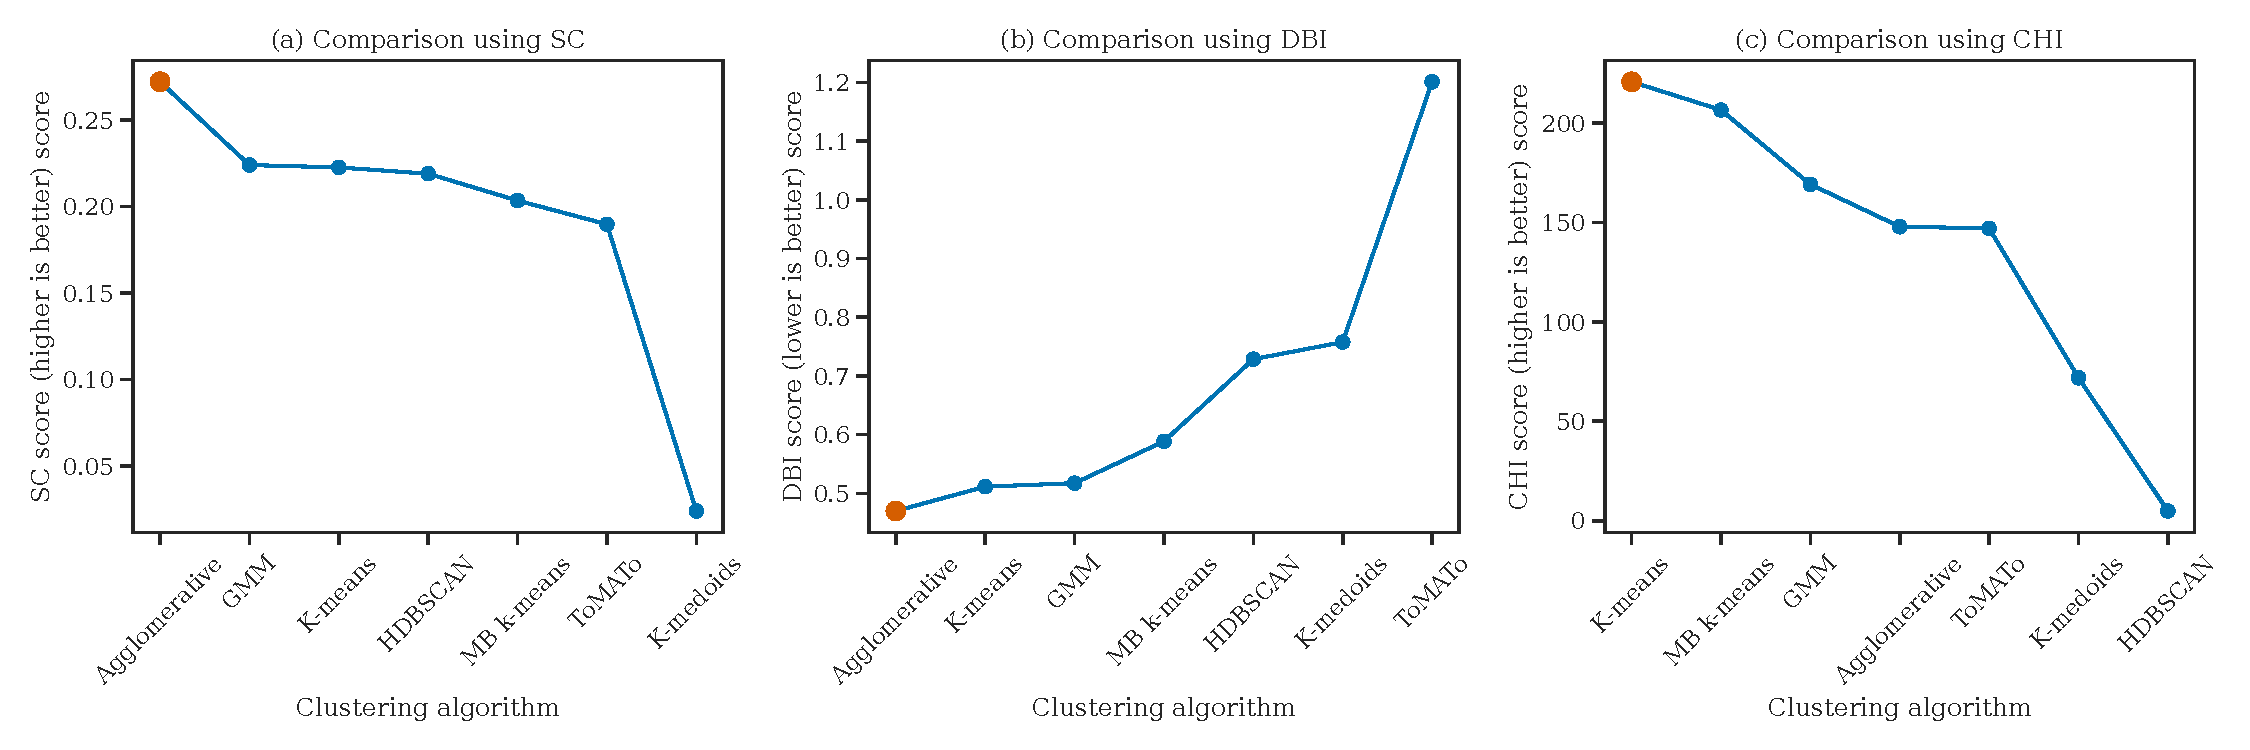
\includegraphics[width=\textwidth]{thesis/figures/cluster-analysis-comparison-internal-cluster-validation.pdf}
    \caption{Comparison of internal cluster validation results from clustering algorithms trained on word embeddings from the SGNS-enwiki model. The red dot in each plot denotes the most optimal value.}
    \label{fig:cluster-analysis-comparison-internal-cluster-validation}
\end{figure}

We will now look at the initial grid search result using the agglomerative clustering algorithm to deepen our understanding of the results. We visualize the results in \cref{fig:cluster-analysis-agglomerative-internal-cluster-validation}, and we notice that by using the single linkage criterion, we get relatively poor results. For the remaining criteria, we observe that we get more or less the same results, with the ward criterion being slightly ahead of the rest. By inspecting the best value for the number of clusters for each internal cluster validation method in \cref{fig:cluster-analysis-agglomerative-internal-cluster-validation}, we observe that the DBI and the CHI gives misleading results, while the SC is more meaningful. In particular, the DBI prefers to have the largest number of clusters, that is, 8000 clusters. We inspected the clusters and observed that 6350 of the words are in clusters of size 1. This means that the DBI is not particularly well suited for choosing the number of clusters, as it prefers to have the most clusters. This is illustrated in \cref{fig:cluster-analysis-agglomerative-internal-cluster-validation} (b). Using the CHI, we observe that it prefers to have the least number of clusters, namely 2. We inspected this result and noticed that in the first cluster, there was only a single word, while the second cluster had the remaining 9999 words. In other words, this indicates that the CHI is also not particularly well suited for choosing the number of clusters. Finally, using the SC, shown in \cref{fig:cluster-analysis-agglomerative-internal-cluster-validation} (a), we observe that the preferred number of clusters lie around 3000 to 6000. We inspected the number of clusters as preferred by average, complete and ward linkage clustering and observed that they made sense, as there was more variety in the cluster sizes and the number of clusters having the specific cluster sizes. This indicates that the most preferable number of clusters (using SC) should lie in this range (3000 to 6000), and following, we will narrow down the search for the best number of clusters. For the next experiment, we will not include the single linkage clustering criterion, as it performed poorly.
\begin{figure}[H]
    \centering
    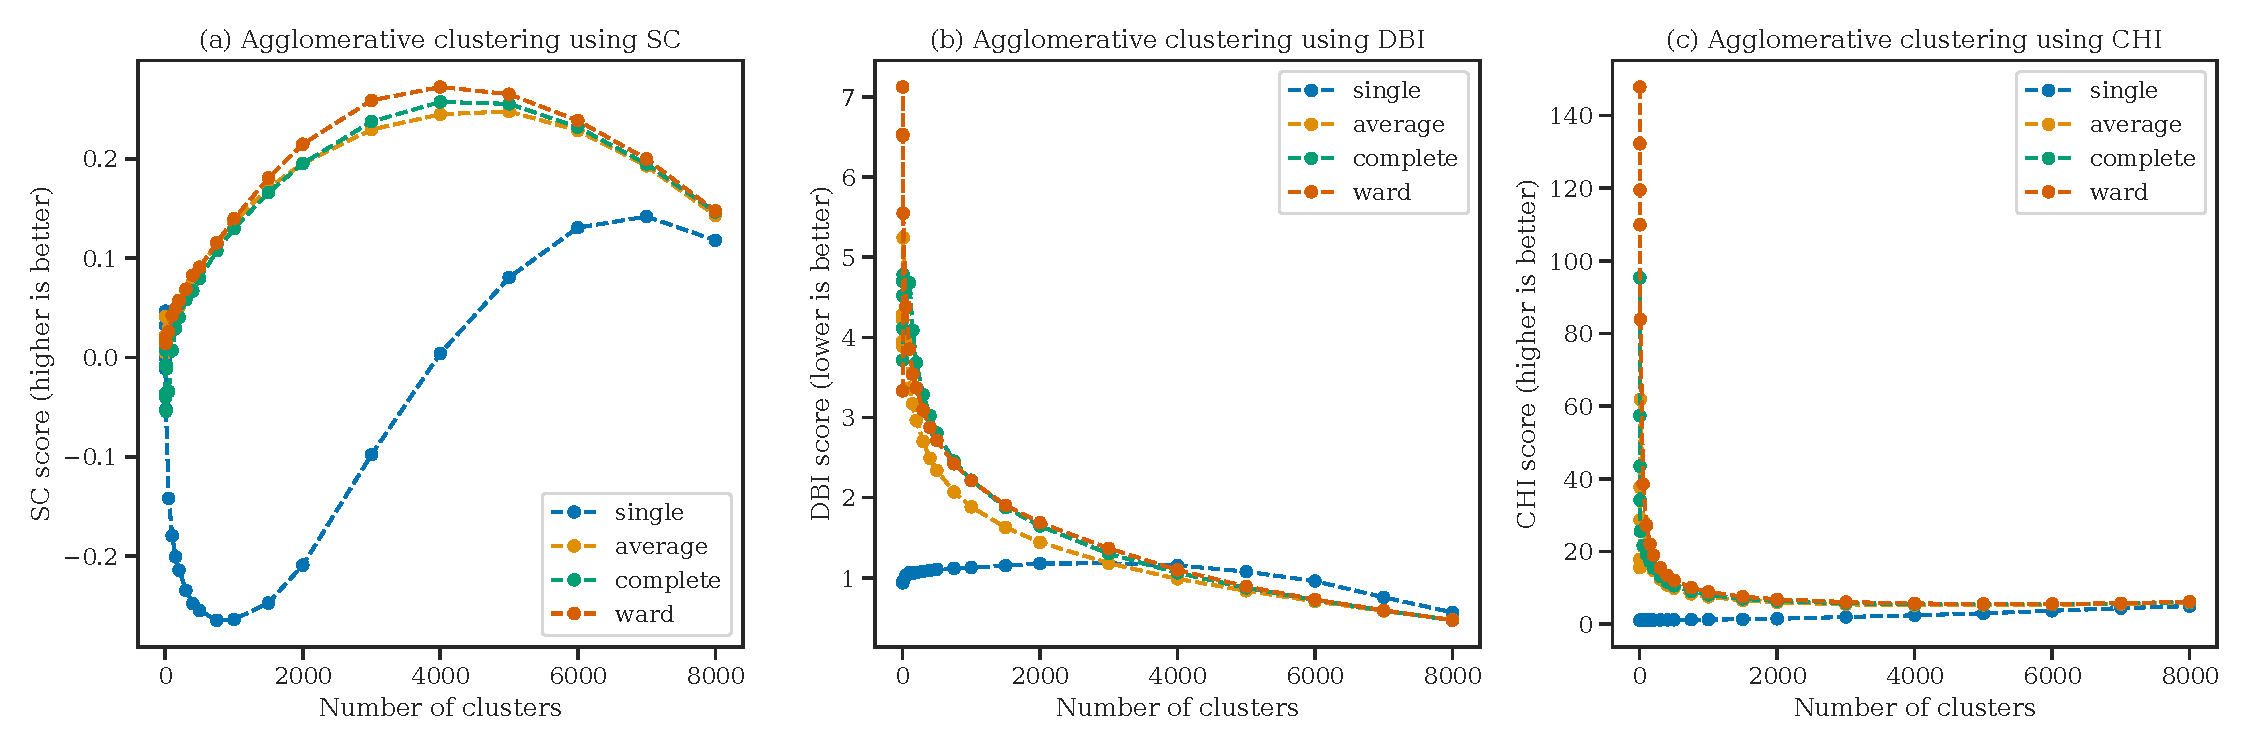
\includegraphics[width=\textwidth]{thesis/figures/cluster-analysis-agglomerative-internal-cluster-validation.pdf}
    \caption{Internal cluster validation results using agglomerative clustering on word embeddings from SGNS-enwiki.}
    \label{fig:cluster-analysis-agglomerative-internal-cluster-validation}
\end{figure}

By narrowing the search to the range of 3000 to 6000 clusters, we find the best number of clusters for each criterion of agglomerative clustering. The narrowed search for the number of clusters is visualized in \cref{fig:cluster-analysis-agglomerative-internal-cluster-validation-narrow}, and we observe that ward linkage clustering with 4104 clusters results in the best clustering. In other words, these results indicate that, by using the ward clustering criterion, we obtain the best clustering of the 10000 most common words from the SGNS-enwiki model.
\begin{figure}[H]
    \centering
    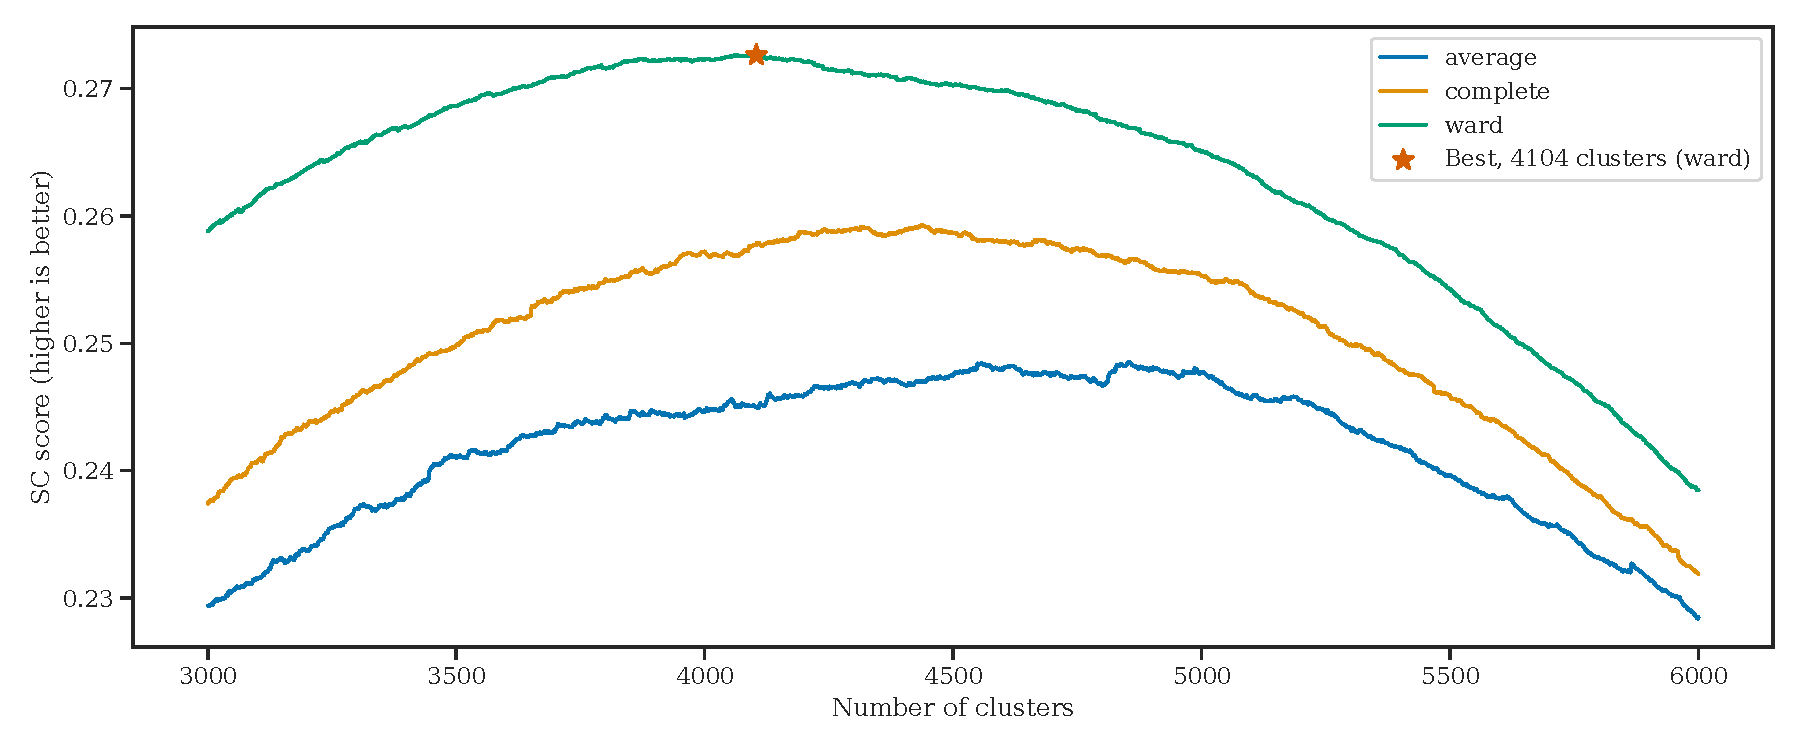
\includegraphics[width=\textwidth]{thesis/figures/cluster-analysis-agglomerative-internal-cluster-validation-narrow.pdf}
    \caption{A number of clusters search using agglomerative clustering and SC, on the range of 3000 to 6000 clusters. Here we see that the ward linkage criterion results in the highest SC score.}
    \label{fig:cluster-analysis-agglomerative-internal-cluster-validation-narrow}
\end{figure}

To deepen our understanding of the clustering result using agglomerative clustering and ward criterion on the word embeddings from SGNS-enwiki, we investigated the words falling into the 4104 clusters. In particular, we looked at the 10 largest and smallest clusters. We restricted the smallest clusters to contain at least 2 words, ensuring that we do not get clusters consisting of single words. In the top 10 largest clusters, we mostly saw names such as "Smith", "Wilson", or "Taylor" clustered together. We also saw the clustering of words representing numbers, e.g. "forty-five", "thirty-two" or "fifty-one", and the clustering of family-related words, e.g. "father", "son" and "brother". The top 10 smallest clusters mostly consisted of words that were strongly related to one another, such as "Adam" and "Noah", "card" and "cards", or "interior" and "exterior". We visualize some of the largest and smallest clusters in \cref{fig:cluster-analysis-agglomerative-2d-umap-top-clusters}, using a 2-dimensional UMAP (\cref{sec:umap}) embedding. To create the UMAP embedding, we used the \path{umap-learn} Python package \cite{mcinnes2018umap-software} and the default hyperparameterization. In \cref{fig:cluster-analysis-agglomerative-2d-umap-top-clusters}, we see that the clusters are widely spread all over the UMAP embedding. In addition to this, the UMAP embedding suggests that there are more clusters throughout the word embeddings, which the clustering algorithms were unable to pick up (when evaluated using internal cluster validation methods). We will investigate this further, and in the next subsection, we will look at the clustering of distinct word groups. In particular, we will see if bigger sets of words cluster together in the UMAP embedding, suggesting that the word embeddings contains a deeper structure.
\begin{figure}
    \centering
    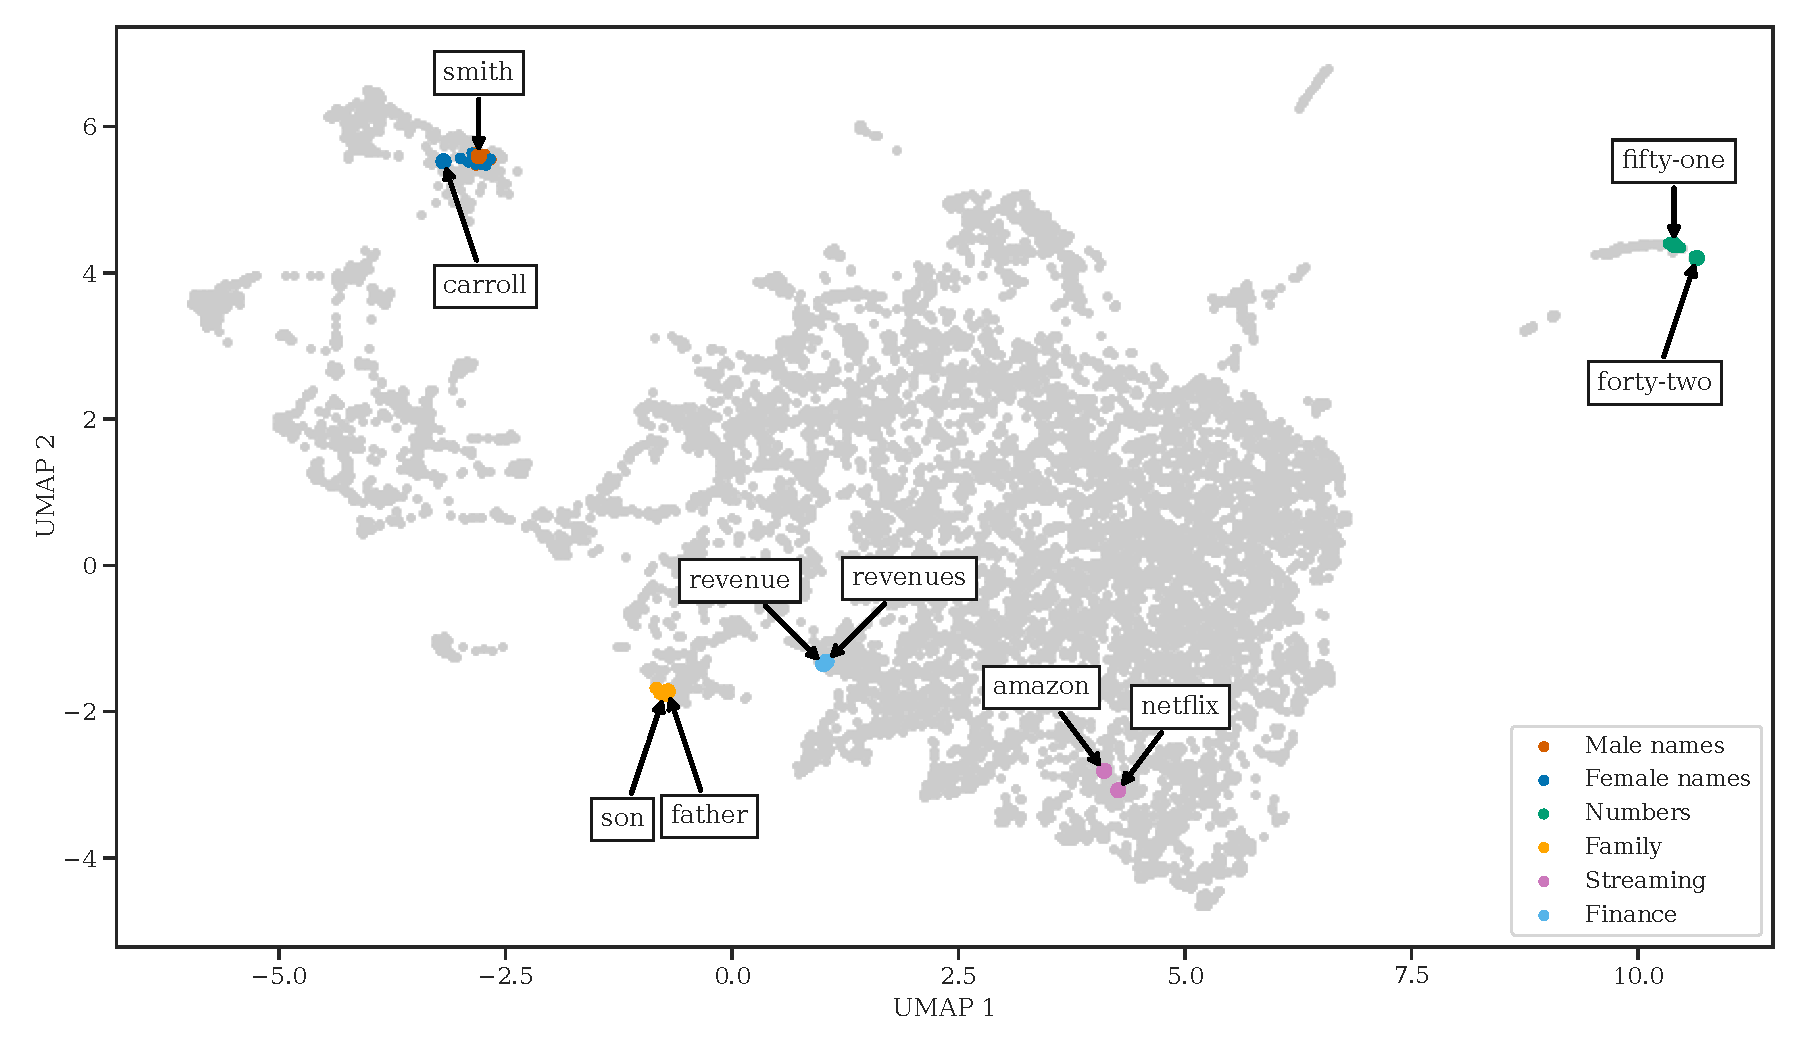
\includegraphics[width=\textwidth]{thesis/figures/cluster-analysis-agglomerative-2d-umap-top-clusters.pdf}
    \caption{2-dimensional UMAP embedding of the 10000 most common words from the SGNS-enwiki model, with some of the largest and smallest clusters outlined.}
    \label{fig:cluster-analysis-agglomerative-2d-umap-top-clusters}
\end{figure}

\subsection{Clustering word groups}
\label{sec:clustering-word-groups}
In this subsection, we will investigate the effect of clustering in the 2-dimensional UMAP embedding of the 10000 most common words of the SGNS-enwiki model, using distinct groups of words. In particular, we will cluster words related to countries/capitals, numbers, names (fore- and surnames) and food. Before performing the clustering, we first prepare the data used for the analysis. The countries/capitals data was retrieved from \cite{GeoNames}, where we used their API to fetch countries and their capital, resulting in 217 pairs of countries and capitals that were in the SGNS-enwiki vocabulary. The number data was generated by converting numbers to their string representation. We converted the numbers from zero to one trillion, resulting in 105 number-related words. The forenames data was retrieved from \cite{SSABabyNames}, where we used the top 1000 baby names from 2019. The surnames data was retrieved from \cite{CensusSurnames}, and we used the top 1000 surnames from 2010. Finally, the food data was retrieved from \cite{FoodIngredientList}, where we used the 250 most common ingredient words. We visualize the largest word group clusters falling into the 10000 most common words of the word embeddings from the SGNS-enwiki in \cref{fig:word-cluster-all-groups}, where we use a 2-dimensional UMAP embedding. In \cref{fig:word-cluster-all-groups}, we observe that two well-separated clusters are forming in the UMAP embedding, being the names and numbers word groups. We also see that the countries and food groups are more spread out in the embedding.
\begin{figure}[H]
    \centering
    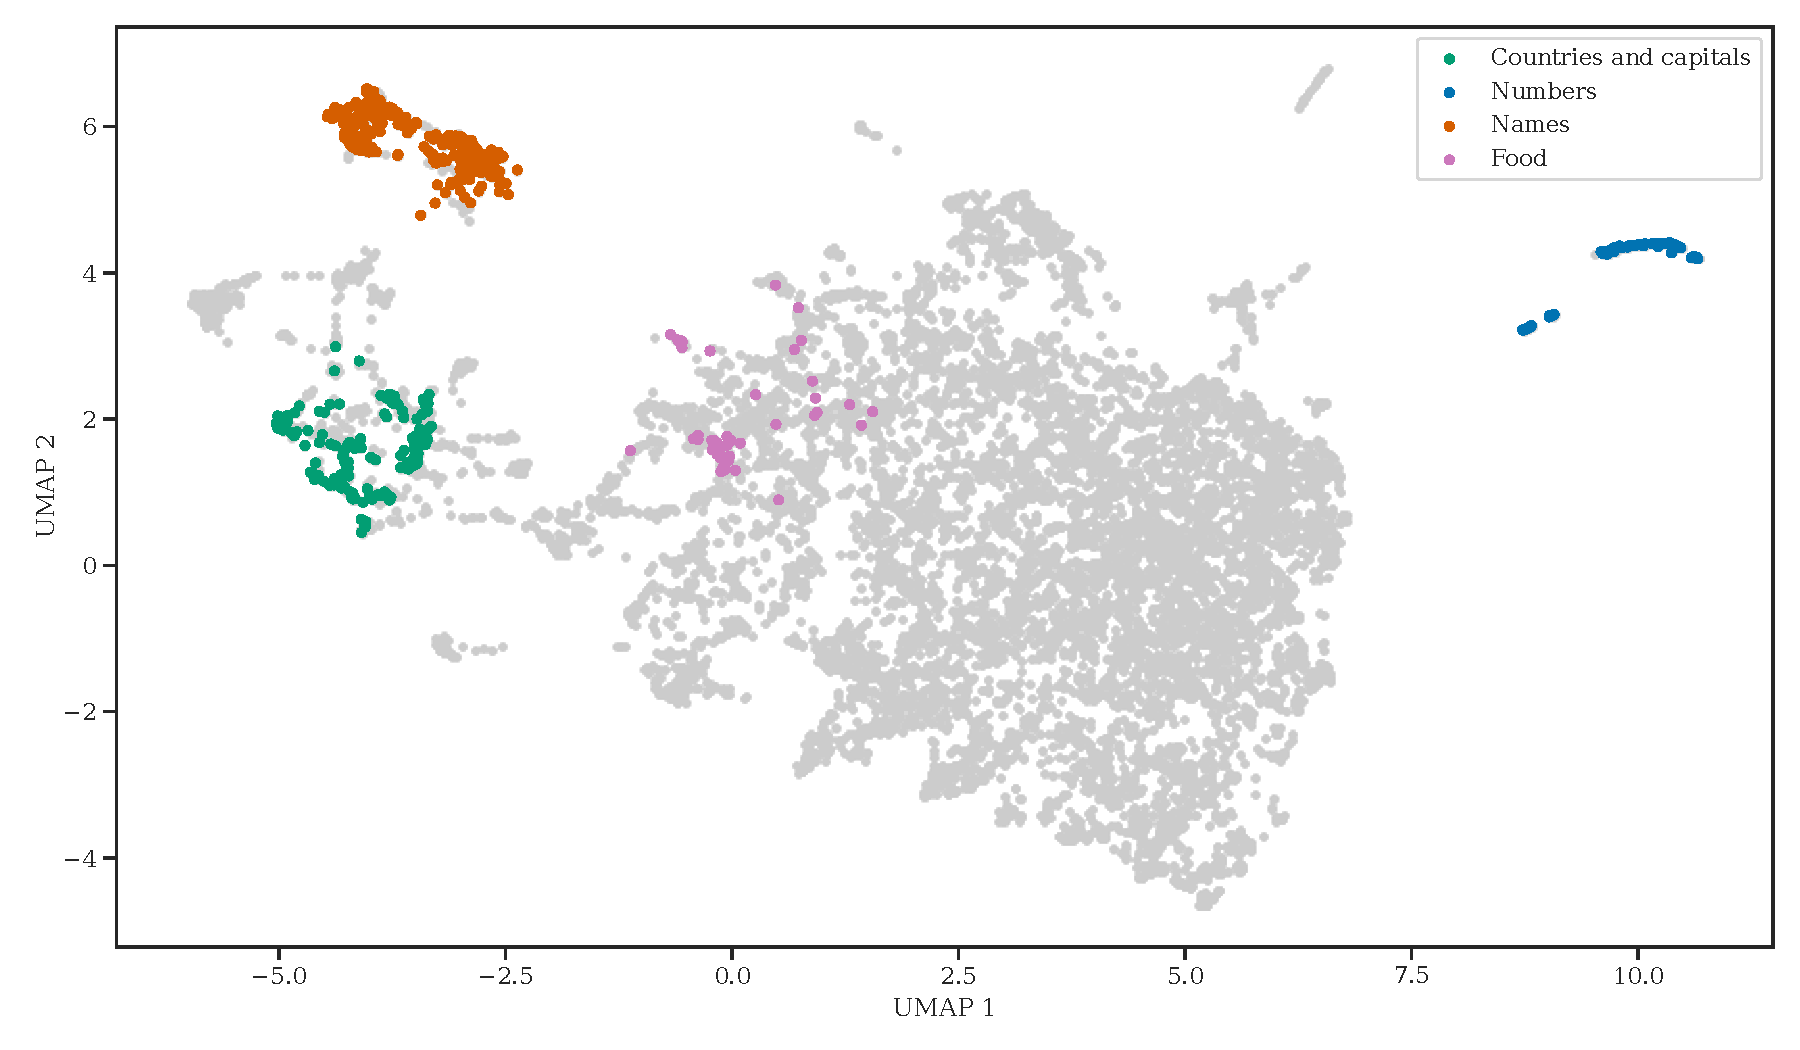
\includegraphics[width=\textwidth]{thesis/figures/word-cluster-all-groups.pdf}
    \caption{2-dimensional UMAP embedding of the 10000 most common words from the SGNS-enwiki model, with word groups outlined.}
    \label{fig:word-cluster-all-groups}
\end{figure}

In \cref{fig:word-cluster-all-groups}, we outline the largest clusters of the word groups and discard words falling out of the largest clusters. By including words that are outside the largest clusters, we saw that, in particular, the names word group is spread throughout the word embedding, as the data we used contained fore- and surnames of common words, such as "joy", "page" or "good". We illustrate this behaviour in \cref{fig:word-cluster-all-groups-emphasis-plots}, where we outline the four different word groups. In \cref{fig:word-cluster-all-groups-emphasis-plots} (a), we see that the country and capital words are mostly clustered to the middle left, with some capitals falling out of the bigger cluster. The "Stanley" and "Hamilton" capital cities are also used as names, as indicated in \cref{fig:word-cluster-all-groups-emphasis-plots} (c). For the numbers, we observe that most number-related words are clustered to the right, clearly separated from the rest of the words. However, we also observe that words such as "million", "billion" and "trillion" are clustered together outside the numbers cluster to the right. By inspection, we observed that the "million", "billion" and "trillion" words were, in fact, close to other financial words, such as "banks", "wealth" or "economics". In \cref{fig:word-cluster-all-groups-emphasis-plots} (c), we see that the fore- and surnames are clustered to the top right, in addition to being spread throughout the UMAP embedding. We also observe a small cluster of woman names forming, containing the names "Diana" and "Isabella". Lastly, we see that food-related words in \cref{fig:word-cluster-all-groups-emphasis-plots} (d) are slightly clustered around the words "egg" and "cheese", but also spread around the UMAP embedding. An interesting observation is the word "apple", which is both a fruit and a technology company. In this case, the word apple refers to the company Apple Inc., as we also saw earlier in \cref{table:word2vec-nearest-neighbours-words}.
\begin{figure}[H]
    \centering
    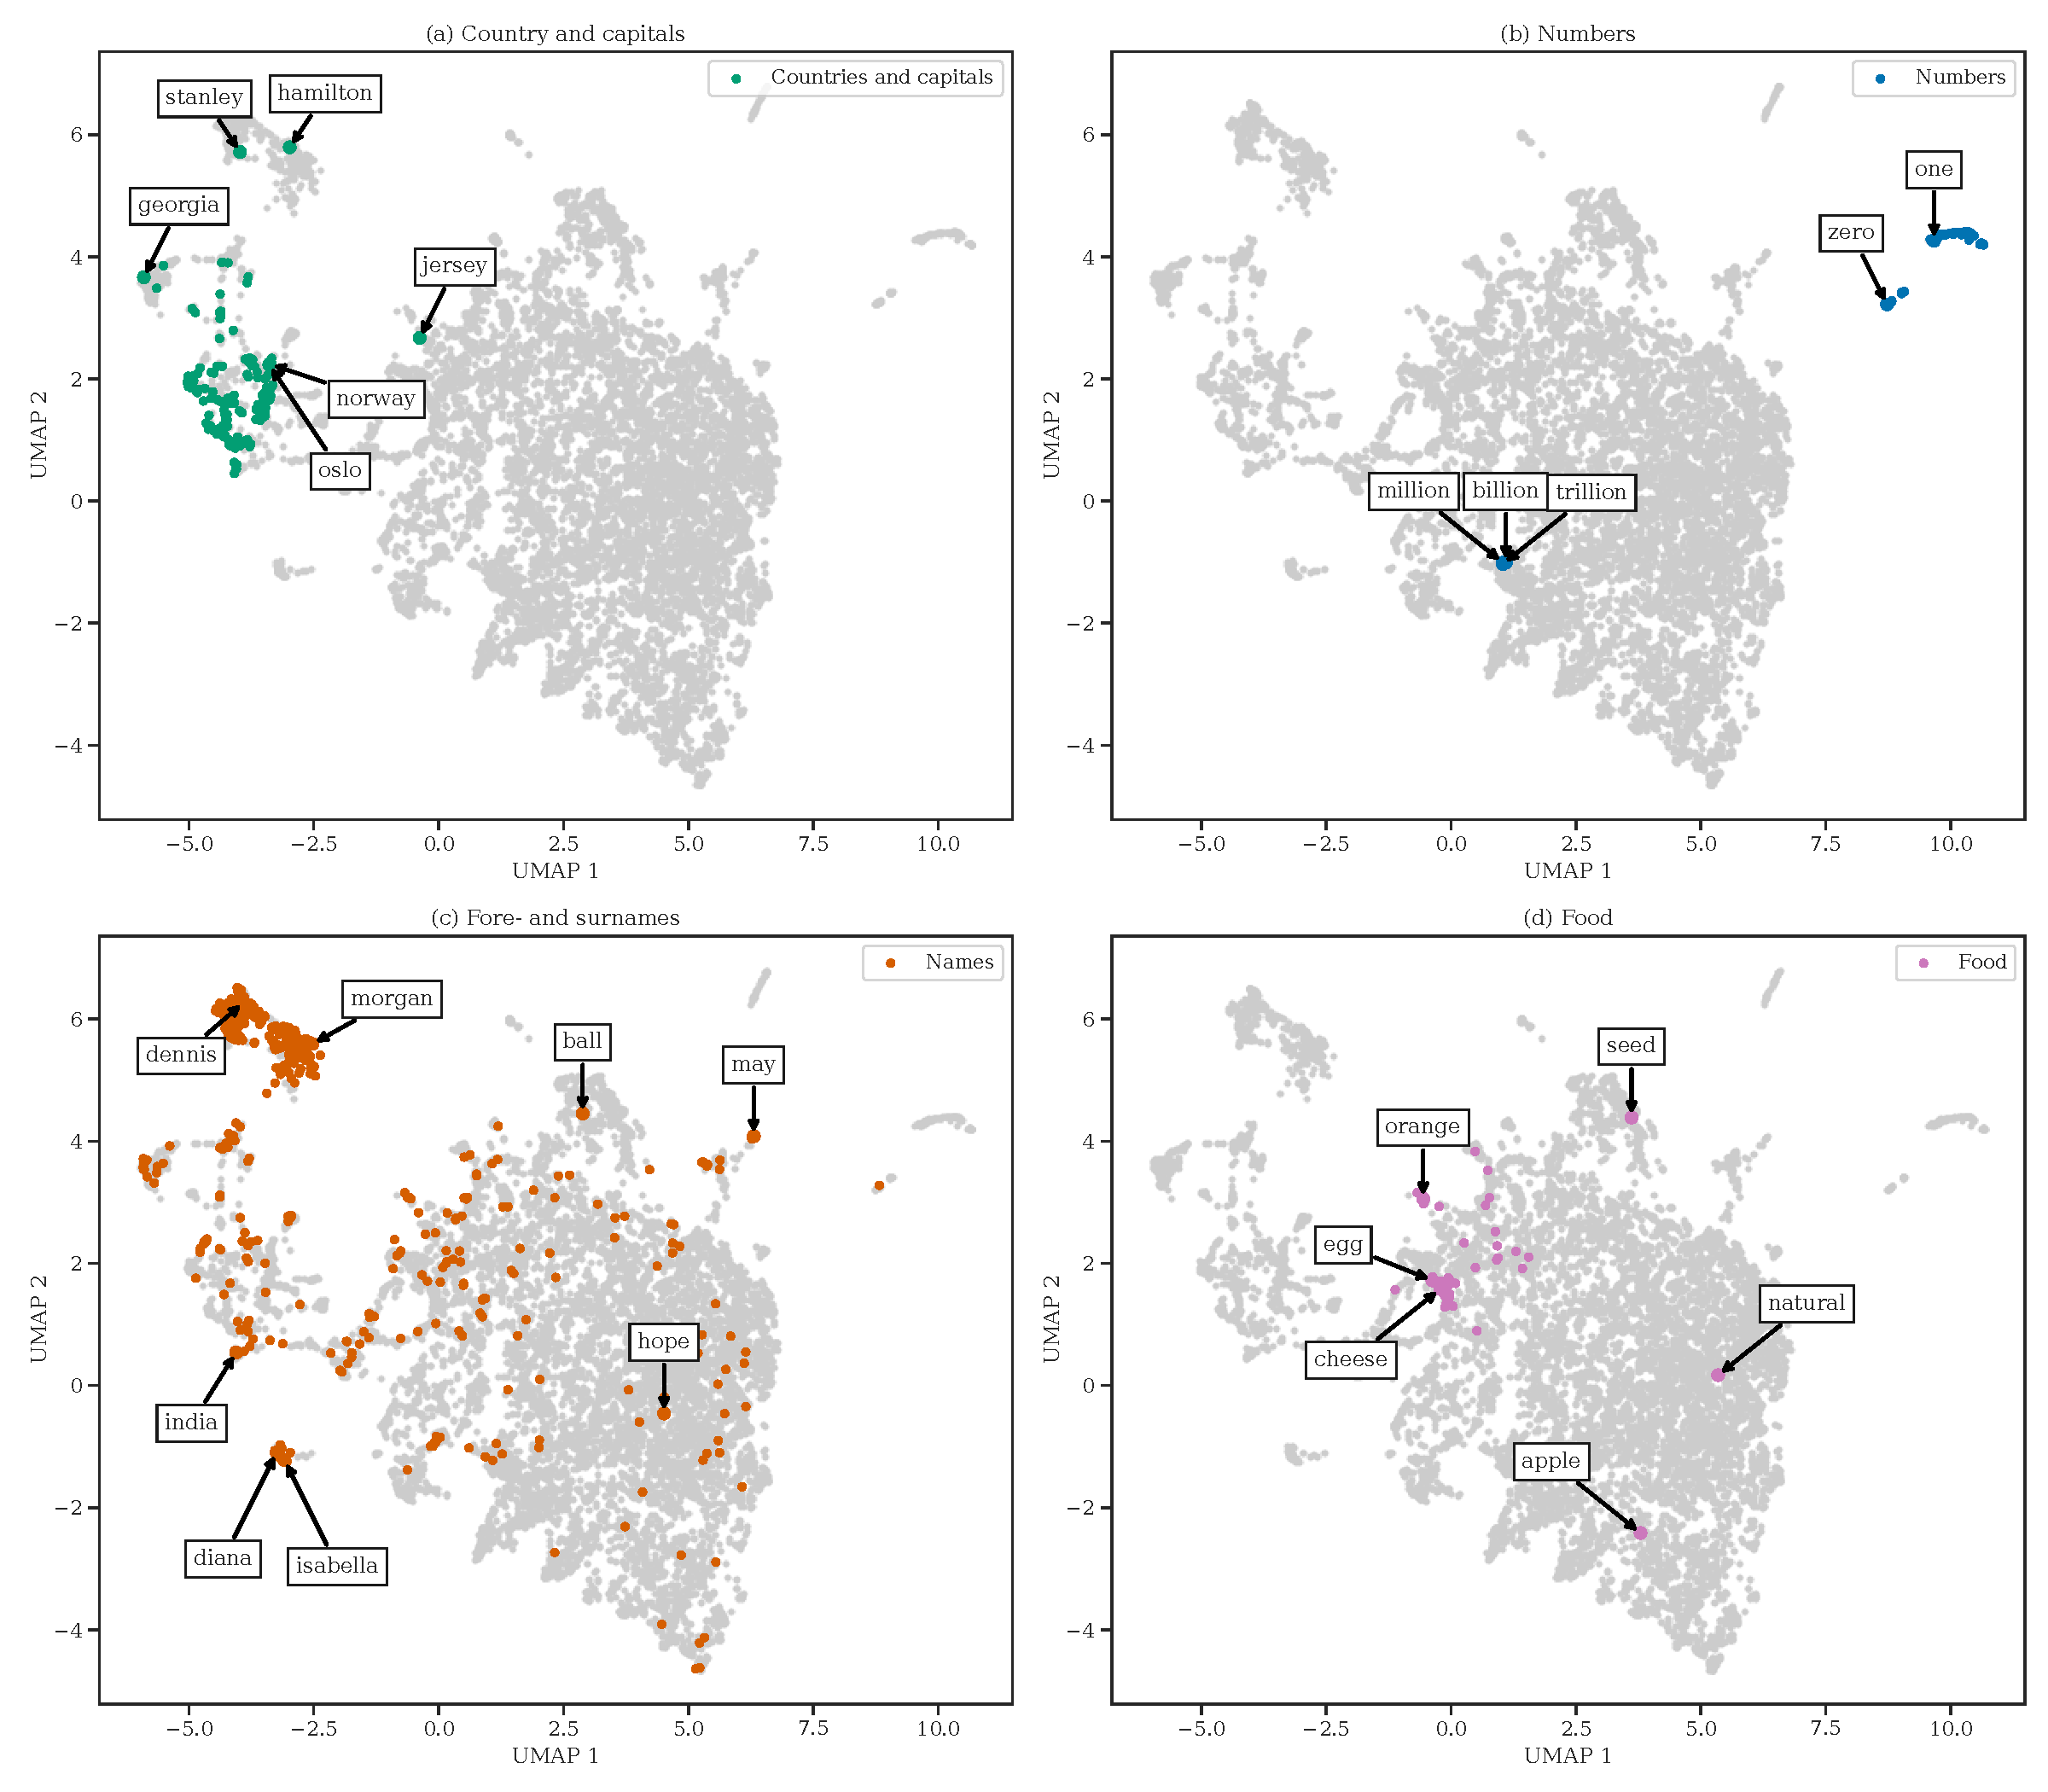
\includegraphics[width=\textwidth]{thesis/figures/word-cluster-all-groups-emphasis-plots.pdf}
    \caption{2-dimensional UMAP embeddings of the 10000 most common words of the SGNS-enwiki model. Here we see four plots, and for each of them, we outline the four different word groups.}
    \label{fig:word-cluster-all-groups-emphasis-plots}
\end{figure}

To further develop our understanding of the SGNS-enwiki word embeddings, we will analyze two of the previous word groups. In particular, we will perform cluster analysis of the word embeddings of countries/capitals and numbers, where we will use clustering algorithms to cluster the words. We will use the same clustering algorithms specified in \cref{sec:comparing-clustering-algorithms}, in addition to Spectral clustering. To visualize the results, we will use dimensionality reduction algorithms to create 2-dimensional embeddings. We will also use latitude/longitude coordinates of countries to visualize the clustering results using countries/capitals word embeddings.

We analyze the countries and capital word groups separately, as we choose to either identify a country by its name or its capital. Starting with the country word group, we perform cluster analysis. The result of the cluster analysis is summarized in \cref{fig:cluster-analysis-country-word-group-internal-cluster-validation}. There we see a similar result to the result shown in \cref{fig:cluster-analysis-comparison-internal-cluster-validation}, namely that agglomerative clustering is the preferred clustering algorithm.
\begin{figure}[H]
    \centering
    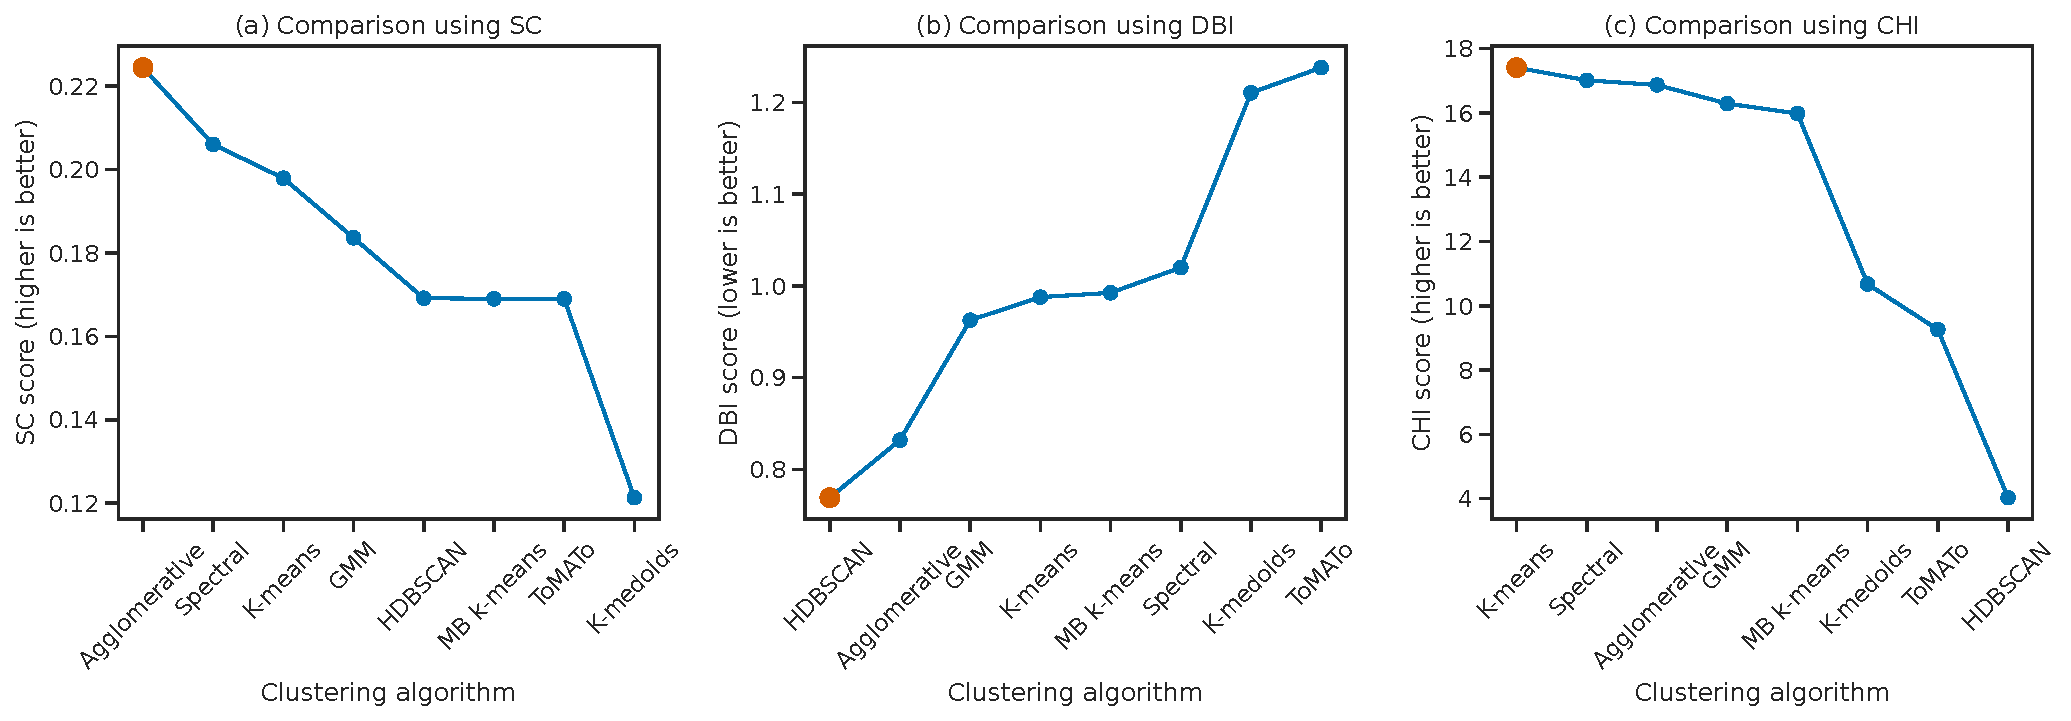
\includegraphics[width=\textwidth]{thesis/figures/cluster-analysis-country-word-group-internal-cluster-validation.pdf}
    \caption{Comparison of internal cluster validation results from clustering algorithms trained on country word embeddings from the SGNS-enwiki model. The red dot in each plot denotes the most optimal value.}
    \label{fig:cluster-analysis-country-word-group-internal-cluster-validation}
\end{figure}

Following, we inspected the scores from the DBI and CHI methods. We observed a similar pattern to the analysis from \cref{sec:comparing-clustering-algorithms}, namely that DBI prefers every word to be in its cluster and CHI prefers to have the smallest number of clusters (i.e. 2). For this reason, we will mainly focus on the results using SC. Using agglomerative clustering, we visualize its result in \cref{fig:cluster-analysis-agglomerative-country-word-group-internal-cluster-validation}. In \cref{fig:cluster-analysis-agglomerative-country-word-group-internal-cluster-validation}, we see similar results to \cref{fig:cluster-analysis-agglomerative-internal-cluster-validation}, namely that ward criterion gives the best clustering when using agglomerative clustering.
\begin{figure}[H]
    \centering
    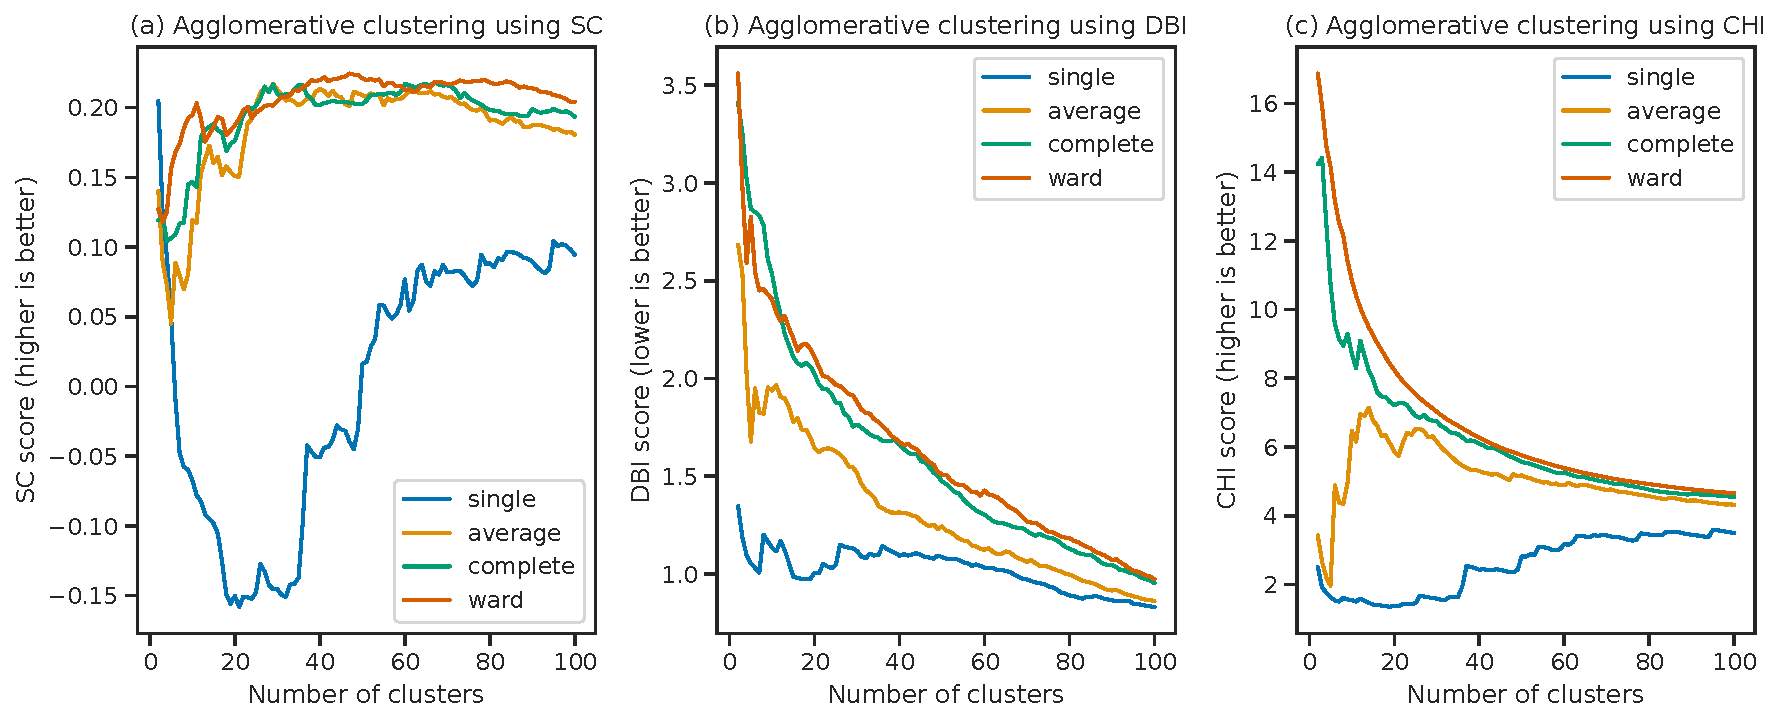
\includegraphics[width=\textwidth]{thesis/figures/cluster-analysis-agglomerative-country-word-group-internal-cluster-validation.pdf}
    \caption{The internal cluster validation results using agglomerative clustering on country word embeddings from SGNS-enwiki.}
    \label{fig:cluster-analysis-agglomerative-country-word-group-internal-cluster-validation}
\end{figure}

The best clustering using SC with agglomerative clustering and ward criterion resulted in 47 clusters. We visualize this result using latitude/longitude coordinates of each country by emphasizing the five largest clusters in \cref{fig:cluster-analysis-agglomerative-country-word-group-top-clusters}, where we see that the top 5 largest clusters are clustered together in the same continent.
\begin{figure}[H]
    \centering
    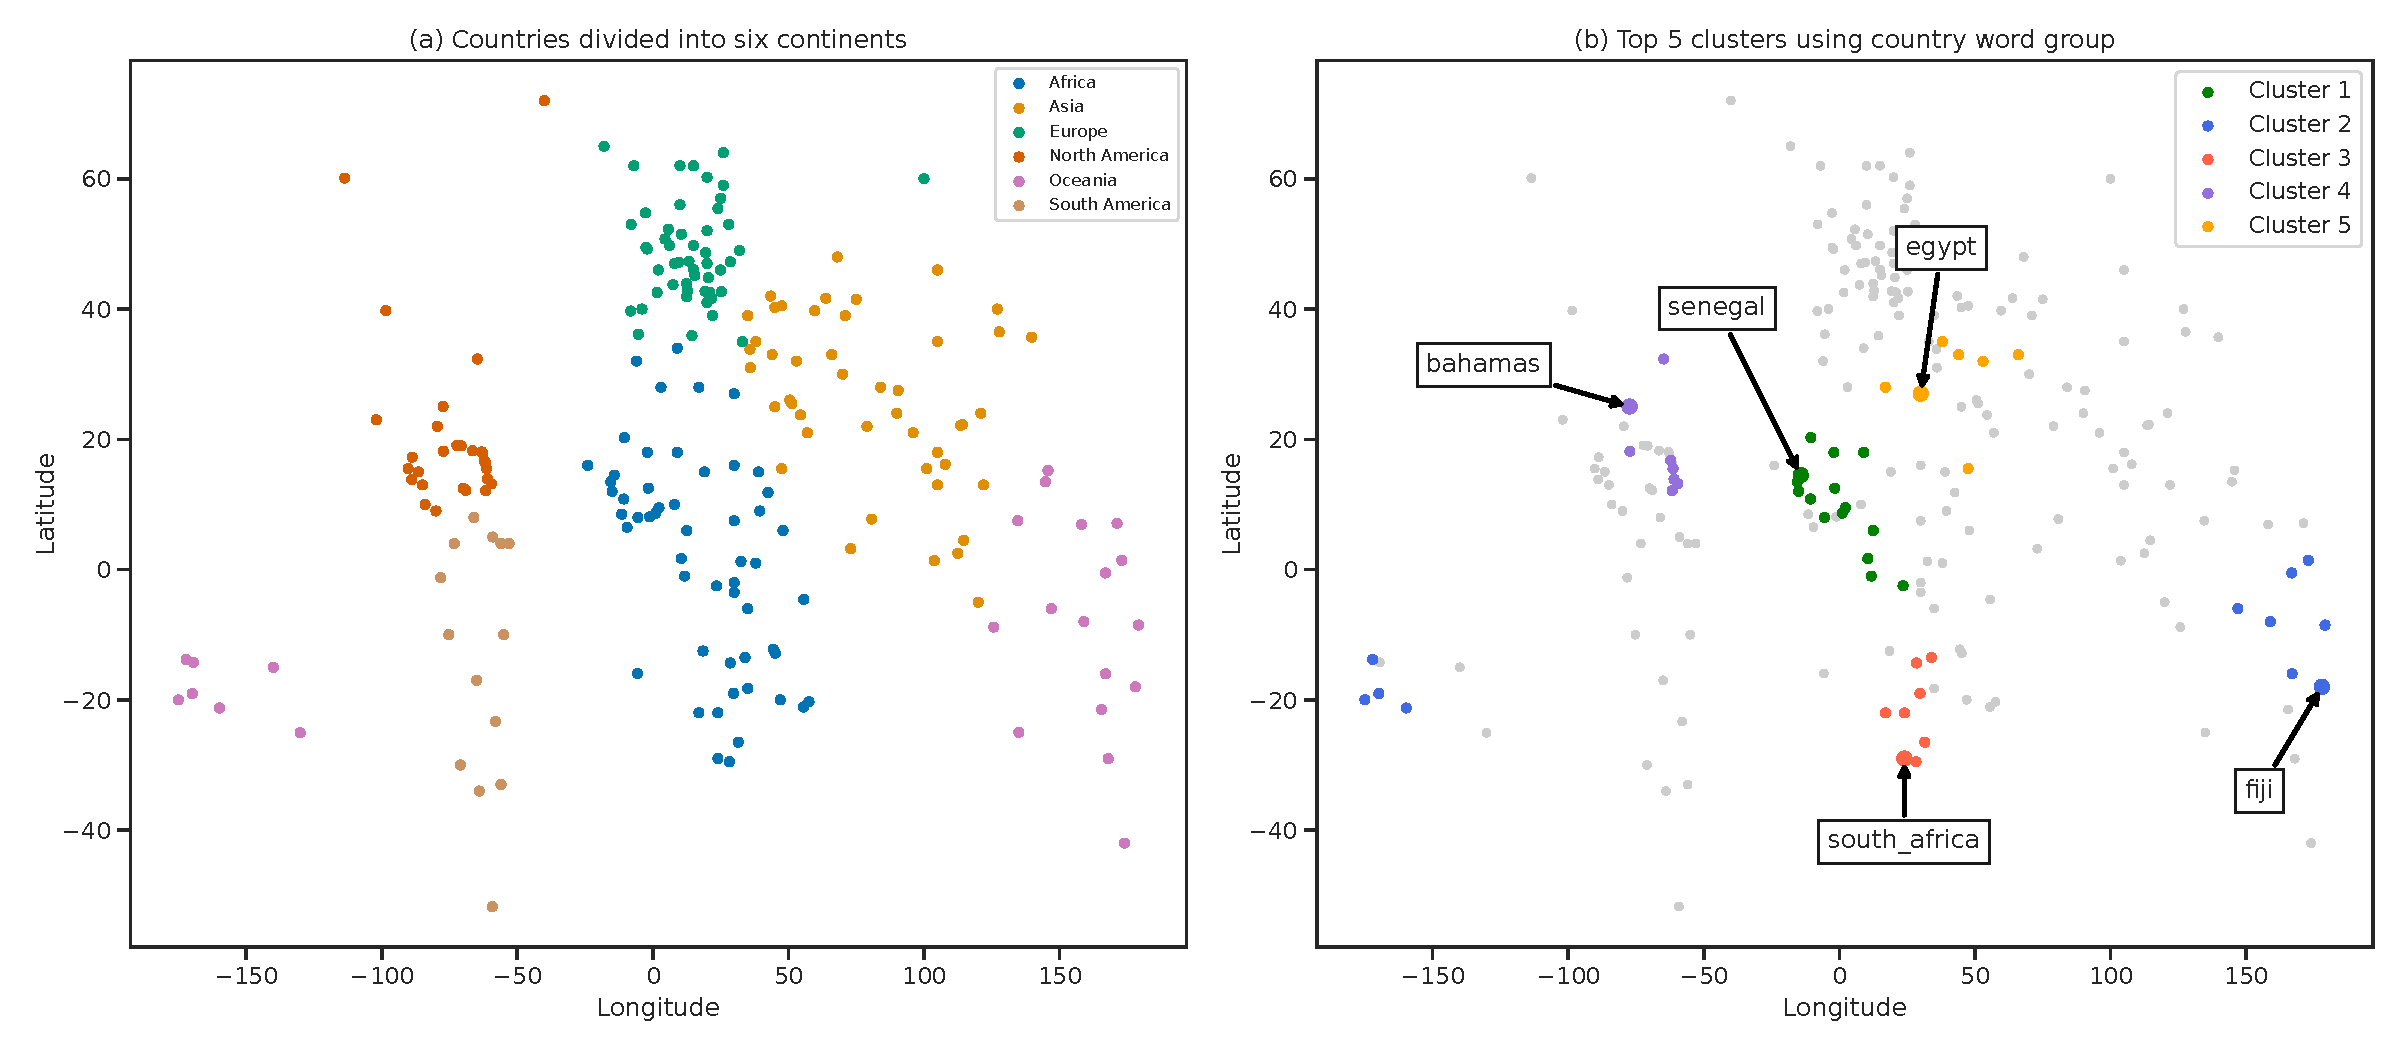
\includegraphics[width=\textwidth]{thesis/figures/cluster-analysis-agglomerative-country-word-group-top-clusters.pdf}
    \caption{A comparison of countries divided into six continents (a) and the top 5 largest clusters from clustering of country word embeddings of the SGNS-enwiki model, using agglomerative clustering and ward criterion. Here we can see that the top 5 largest clusters in (b) correlate well with the continent of the respective countries.}
    \label{fig:cluster-analysis-agglomerative-country-word-group-top-clusters}
\end{figure}

Furthermore, we repeat the cluster analysis using capital to identify each country. That is, we use the word embeddings of the capital words instead of the previously used country word embeddings. The result of the cluster analysis is shown in \cref{fig:cluster-analysis-country-capitals-word-group-internal-cluster-validation}. There we see a similar result to the result shown in both \cref{fig:cluster-analysis-comparison-internal-cluster-validation} and \cref{fig:cluster-analysis-country-word-group-internal-cluster-validation}, namely that agglomerative clustering is the preferred choice of clustering algorithm.
\begin{figure}[H]
    \centering
    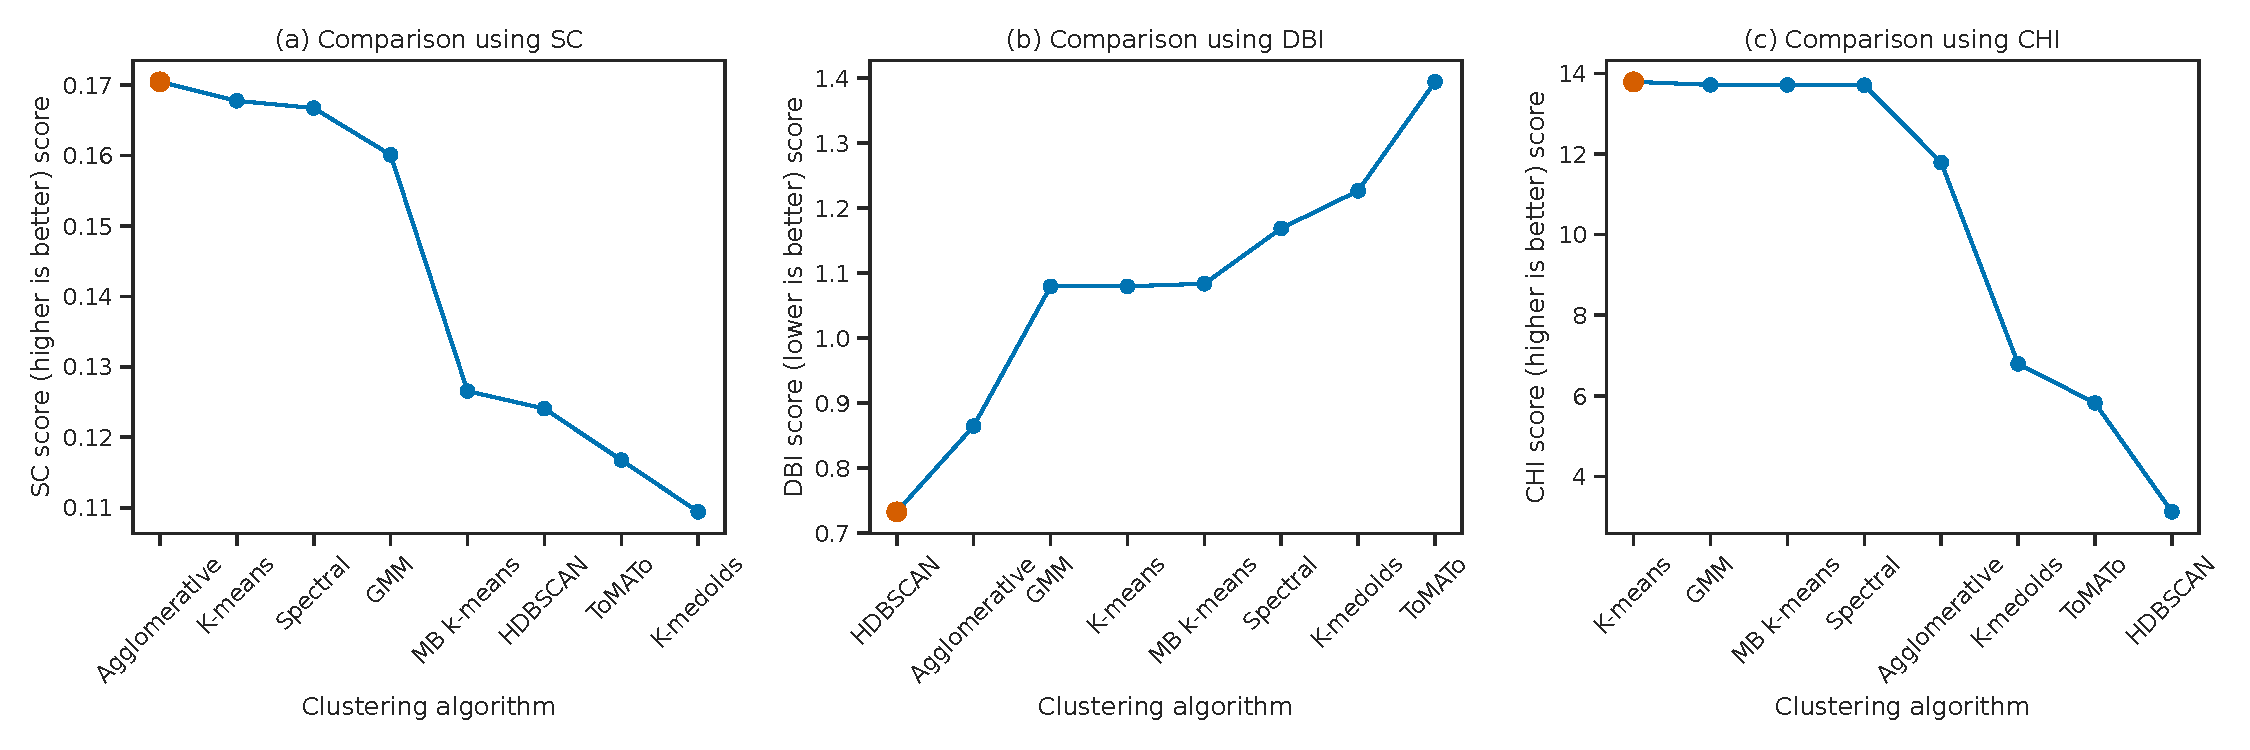
\includegraphics[width=\textwidth]{thesis/figures/cluster-analysis-country-capitals-word-group-internal-cluster-validation.pdf}
    \caption{Comparison of internal cluster validation results from clustering algorithms trained on capital word embeddings from the SGNS-enwiki model. The red dot in each plot denotes the most optimal value.}
    \label{fig:cluster-analysis-country-capitals-word-group-internal-cluster-validation}
\end{figure}

We inspected the scores from the DBI and CHI methods, and similar to the results from \cref{sec:comparing-clustering-algorithms} and the cluster analysis using country word embeddings, we saw that DBI prefers every word to be in its own cluster and CHI prefers to have the smallest number of clusters (i.e. 2). This further strengthens the motivation to use SC over the other methods, and we mainly focus on the results using SC. Using agglomerative clustering, we visualize the results using capital word embeddings in \cref{fig:cluster-analysis-agglomerative-country-capitals-word-group-internal-cluster-validation}. In \cref{fig:cluster-analysis-agglomerative-country-capitals-word-group-internal-cluster-validation}, we see similar results to \cref{fig:cluster-analysis-agglomerative-internal-cluster-validation} and \cref{fig:cluster-analysis-agglomerative-country-word-group-internal-cluster-validation}, namely that ward criterion gives the best clustering when using agglomerative clustering.
\begin{figure}[H]
    \centering
    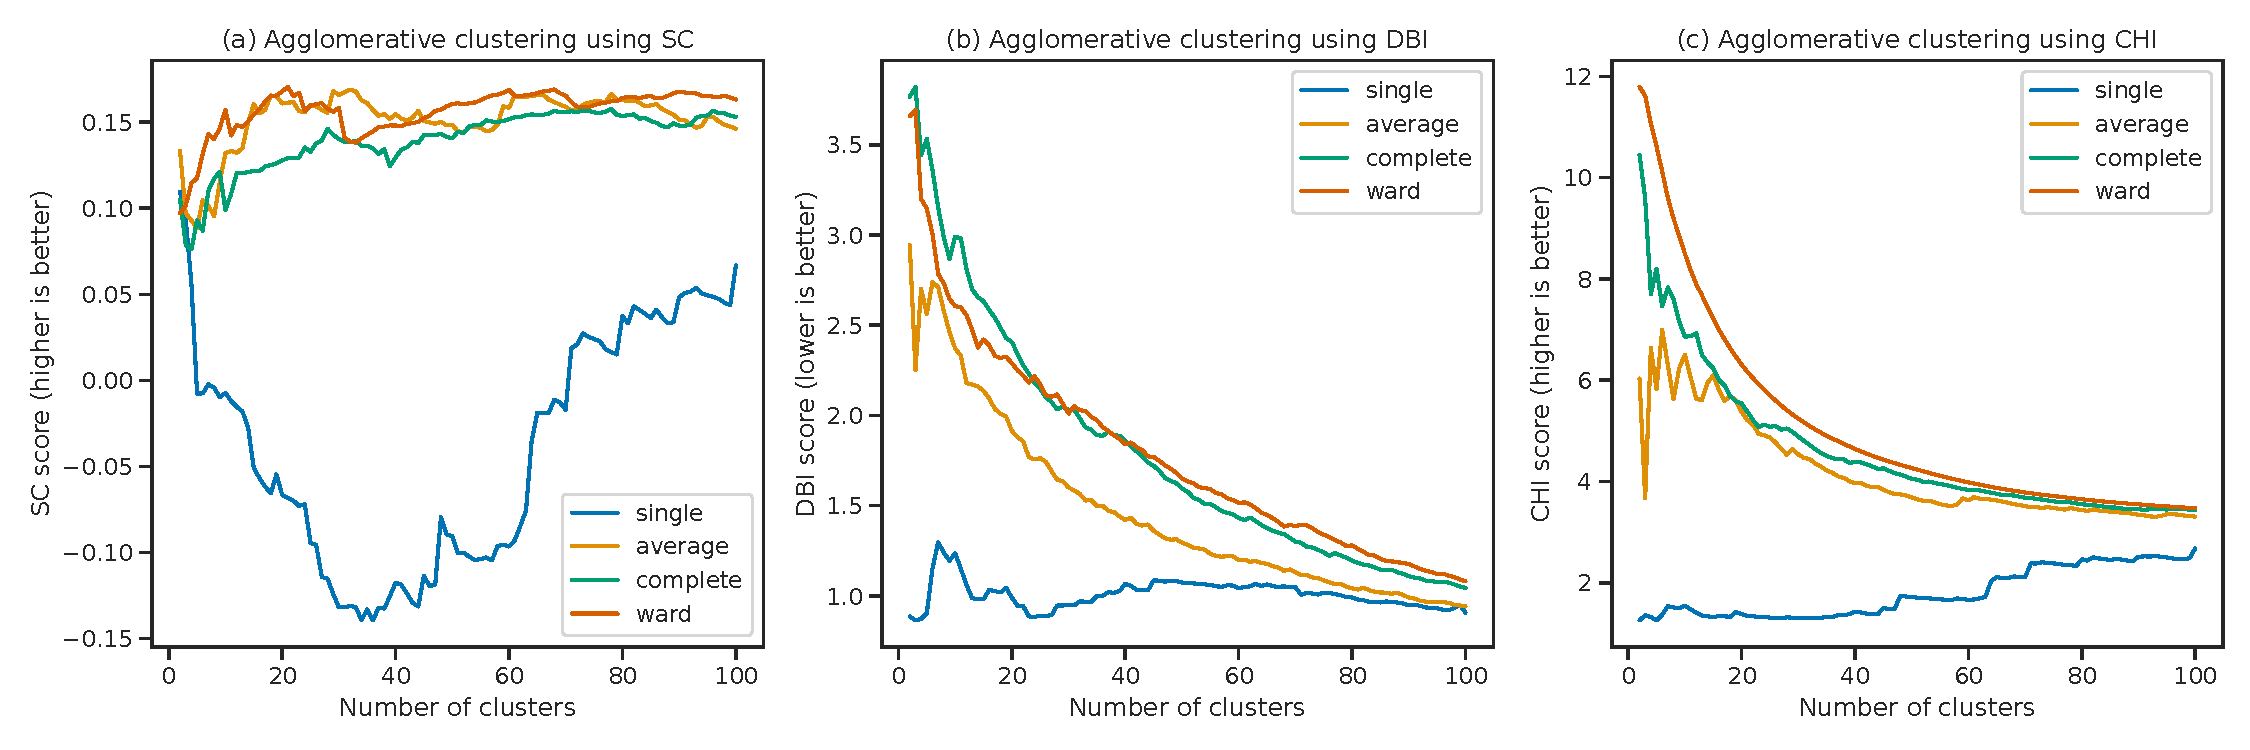
\includegraphics[width=\textwidth]{thesis/figures/cluster-analysis-agglomerative-country-capitals-word-group-internal-cluster-validation.pdf}
    \caption{Internal cluster validation results using agglomerative clustering on capital word embeddings from SGNS-enwiki.}
    \label{fig:cluster-analysis-agglomerative-country-capitals-word-group-internal-cluster-validation}
\end{figure}

The best clustering using SC with agglomerative clustering and ward criterion resulted in 21 clusters. We visualize this result using latitude/longitude coordinates of each country by emphasizing the five largest clusters in \cref{fig:cluster-analysis-agglomerative-country-capitals-word-group-top-clusters}, where we see that we get larger clusters than by using country word embeddings in \cref{fig:cluster-analysis-agglomerative-country-word-group-top-clusters}. Furthermore, we observe that in \cref{fig:cluster-analysis-agglomerative-country-capitals-word-group-top-clusters} (b), the first cluster (green) consists of capitals where the countries are Spanish talking, as outlined by the "Madrid" (Spain), "Mexico City" (Mexico) and "Santiago" (Chile) boxes. The second cluster (blue) in \cref{fig:cluster-analysis-agglomerative-country-capitals-word-group-top-clusters} (b) also correlates well with the Oceanic continent in \cref{fig:cluster-analysis-agglomerative-country-capitals-word-group-top-clusters} (a), while the third (red) and forth (purple) clusters in \cref{fig:cluster-analysis-agglomerative-country-capitals-word-group-top-clusters} (b) seem to capture the African continent very well (Dakar is the capital of Senegal and Pretoria is one of the capitals of South Africa). Lastly, we see that the (yellow) cluster consists of capitals from Eastern Europe, as well as some capitals from Asia.
\begin{figure}[H]
    \centering
    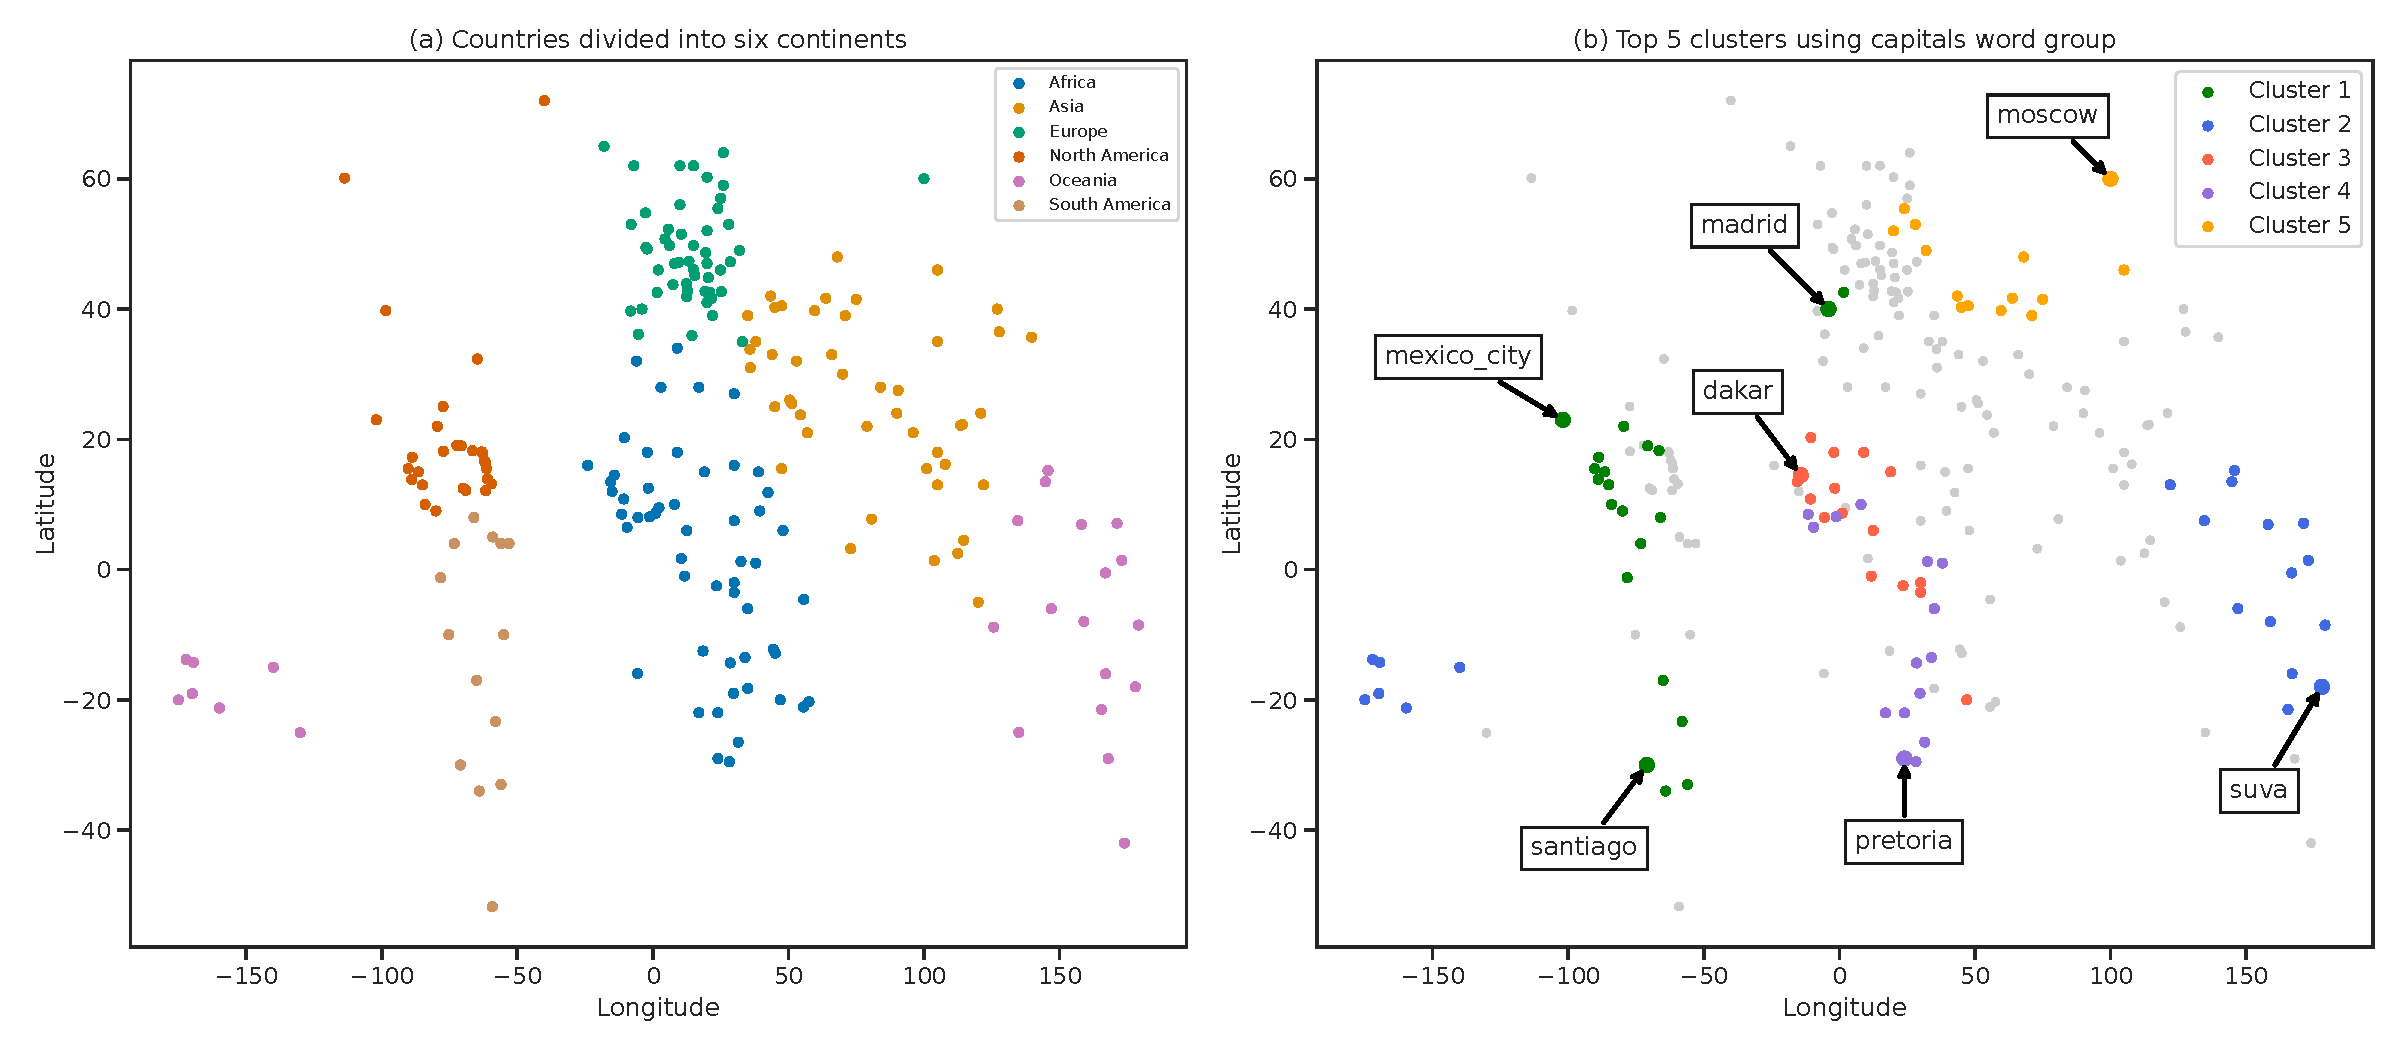
\includegraphics[width=\textwidth]{thesis/figures/cluster-analysis-agglomerative-country-capitals-word-group-top-clusters.pdf}
    \caption{Comparison of countries clustered into their respective continents (a) versus the top 5 largest clusters from clustering of capital word embeddings of the SGNS-enwiki model, using agglomerative clustering and ward criterion. From plot (b) we can see that Spanish speaking countries are clustered together in the first cluster (green), while the other clusters are well clustered with respect to the continent of its country.}
    \label{fig:cluster-analysis-agglomerative-country-capitals-word-group-top-clusters}
\end{figure}

Next, we will perform cluster analysis of number word embeddings in a similar manner to how we performed the cluster analysis of country/capital word embeddings. First, we compared clustering algorithms using internal cluster validation methods, as shown in \cref{fig:cluster-analysis-numbers-word-group-internal-cluster-validation}. In \cref{fig:cluster-analysis-numbers-word-group-internal-cluster-validation}, we see that, overall, the agglomerative clustering algorithm performs the best, when evaluated using internal validation methods.
\begin{figure}[H]
    \centering
    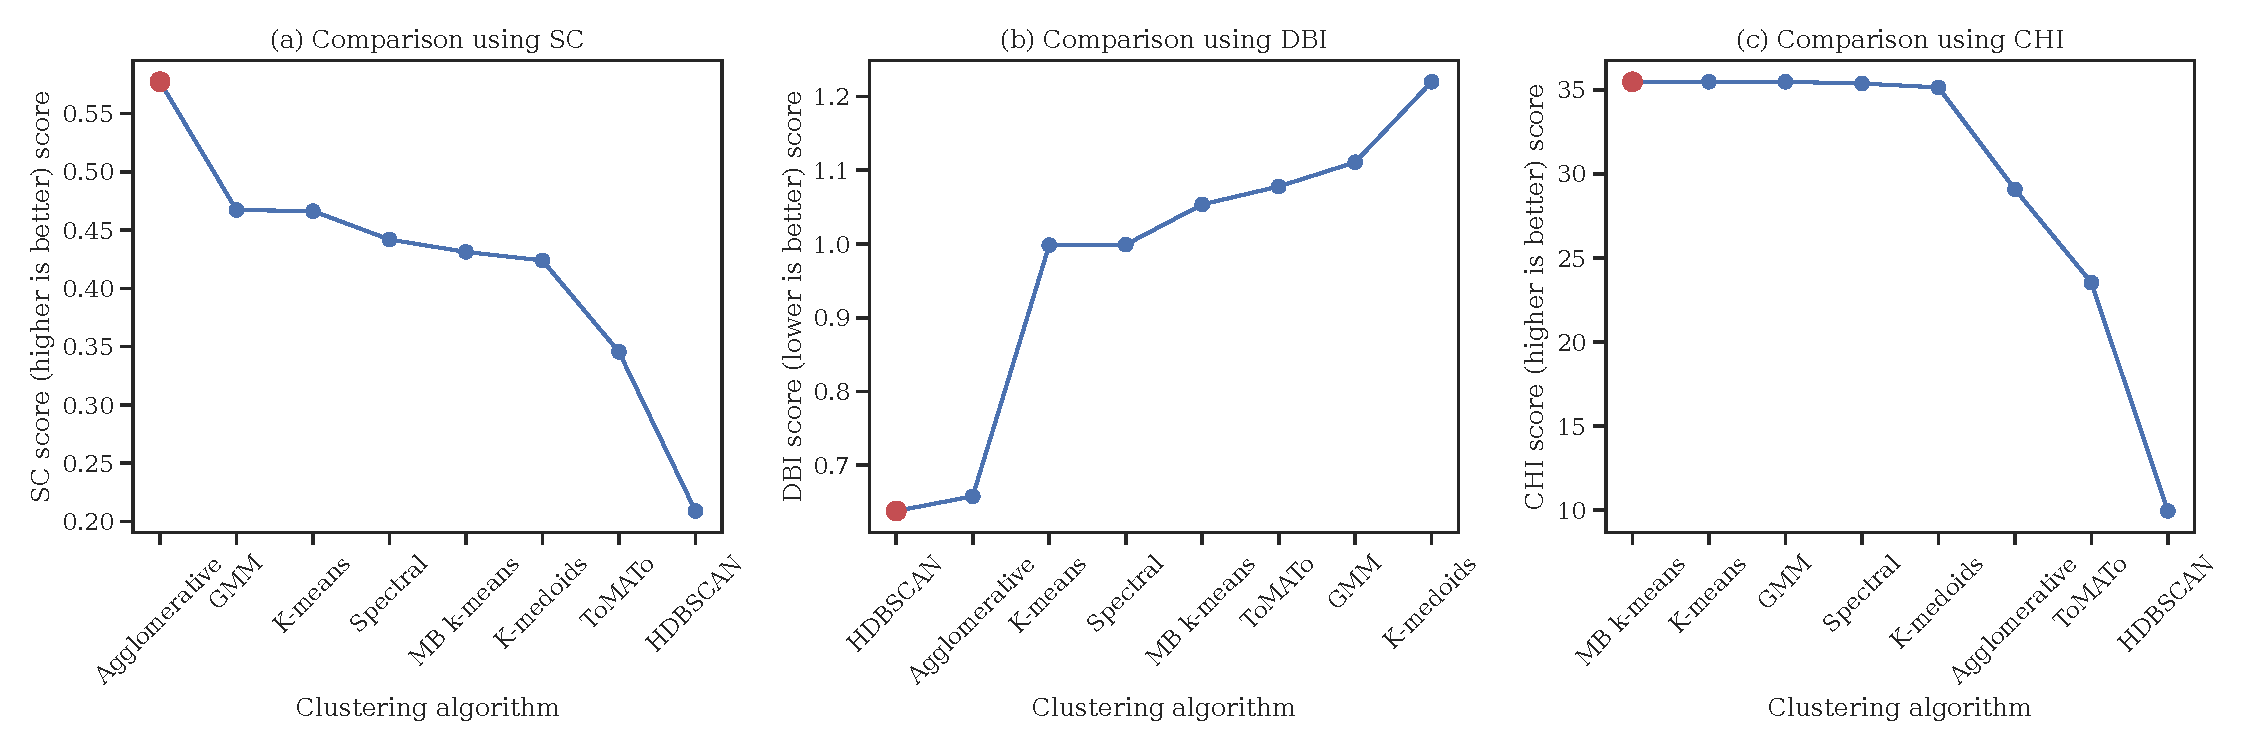
\includegraphics[width=\textwidth]{thesis/figures/cluster-analysis-numbers-word-group-internal-cluster-validation.pdf}
    \caption{Comparison of internal cluster validation results from clustering algorithms trained on number word embeddings from the SGNS-enwiki model. The red dot in each plot denotes the most optimal value.}
    \label{fig:cluster-analysis-numbers-word-group-internal-cluster-validation}
\end{figure}

Furthermore, we will use the agglomerative clustering algorithm to cluster number word embeddings. To find its best criterion and number of clusters, we first visualize its results in \cref{fig:cluster-analysis-agglomerative-numbers-word-group-internal-cluster-validation}. In \cref{fig:cluster-analysis-agglomerative-numbers-word-group-internal-cluster-validation}, we see the internal validation methods prefer different amount of clusters and linkage criteria. In particular, SC prefers complete linkage criterion with 2 clusters, DBI prefers single linkage criterion with 6 clusters, and CHI prefers ward linkage criterion with 3 clusters. In other words, we observe a different behaviour than in the results from the internal cluster validation methods in \cref{sec:comparing-clustering-algorithms} and the country/capital cluster analysis, namely that SC prefers the least amount of clusters, DBI does not prefer the most amount of clusters and CHI does not prefer the least amount of clusters.
\begin{figure}[H]
    \centering
    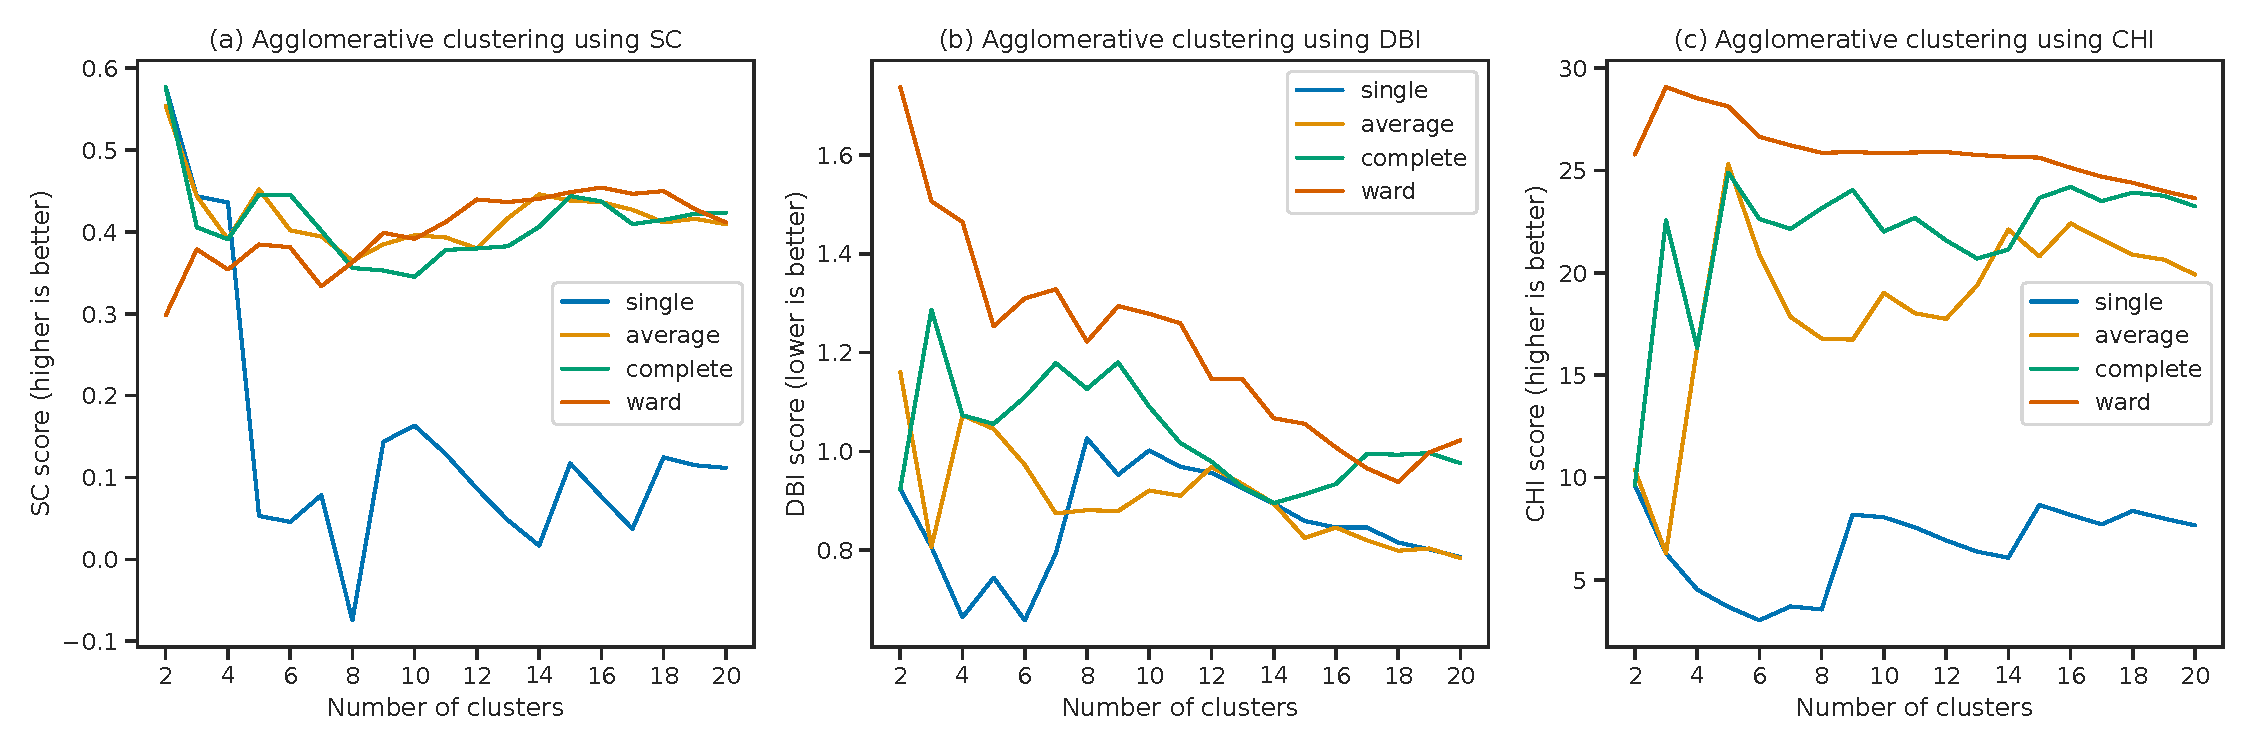
\includegraphics[width=\textwidth]{thesis/figures/cluster-analysis-agglomerative-numbers-word-group-internal-cluster-validation.pdf}
    \caption{Internal cluster validation results using agglomerative clustering on number word embeddings from SGNS-enwiki.}
    \label{fig:cluster-analysis-agglomerative-numbers-word-group-internal-cluster-validation}
\end{figure}

Furthermore, we visualize the best agglomerative clustering result of the number word embeddings as ranked by the internal clustering validation methods in \cref{fig:cluster-analysis-agglomerative-numbers-word-group-internal-cluster-validation-best-2d-pca}, where we use a 2-dimensional PCA embedding. In \cref{fig:cluster-analysis-agglomerative-numbers-word-group-internal-cluster-validation-best-2d-pca}, we see that it is not entirely clear how to cluster the number word embeddings.
\begin{figure}[H]
    \centering
    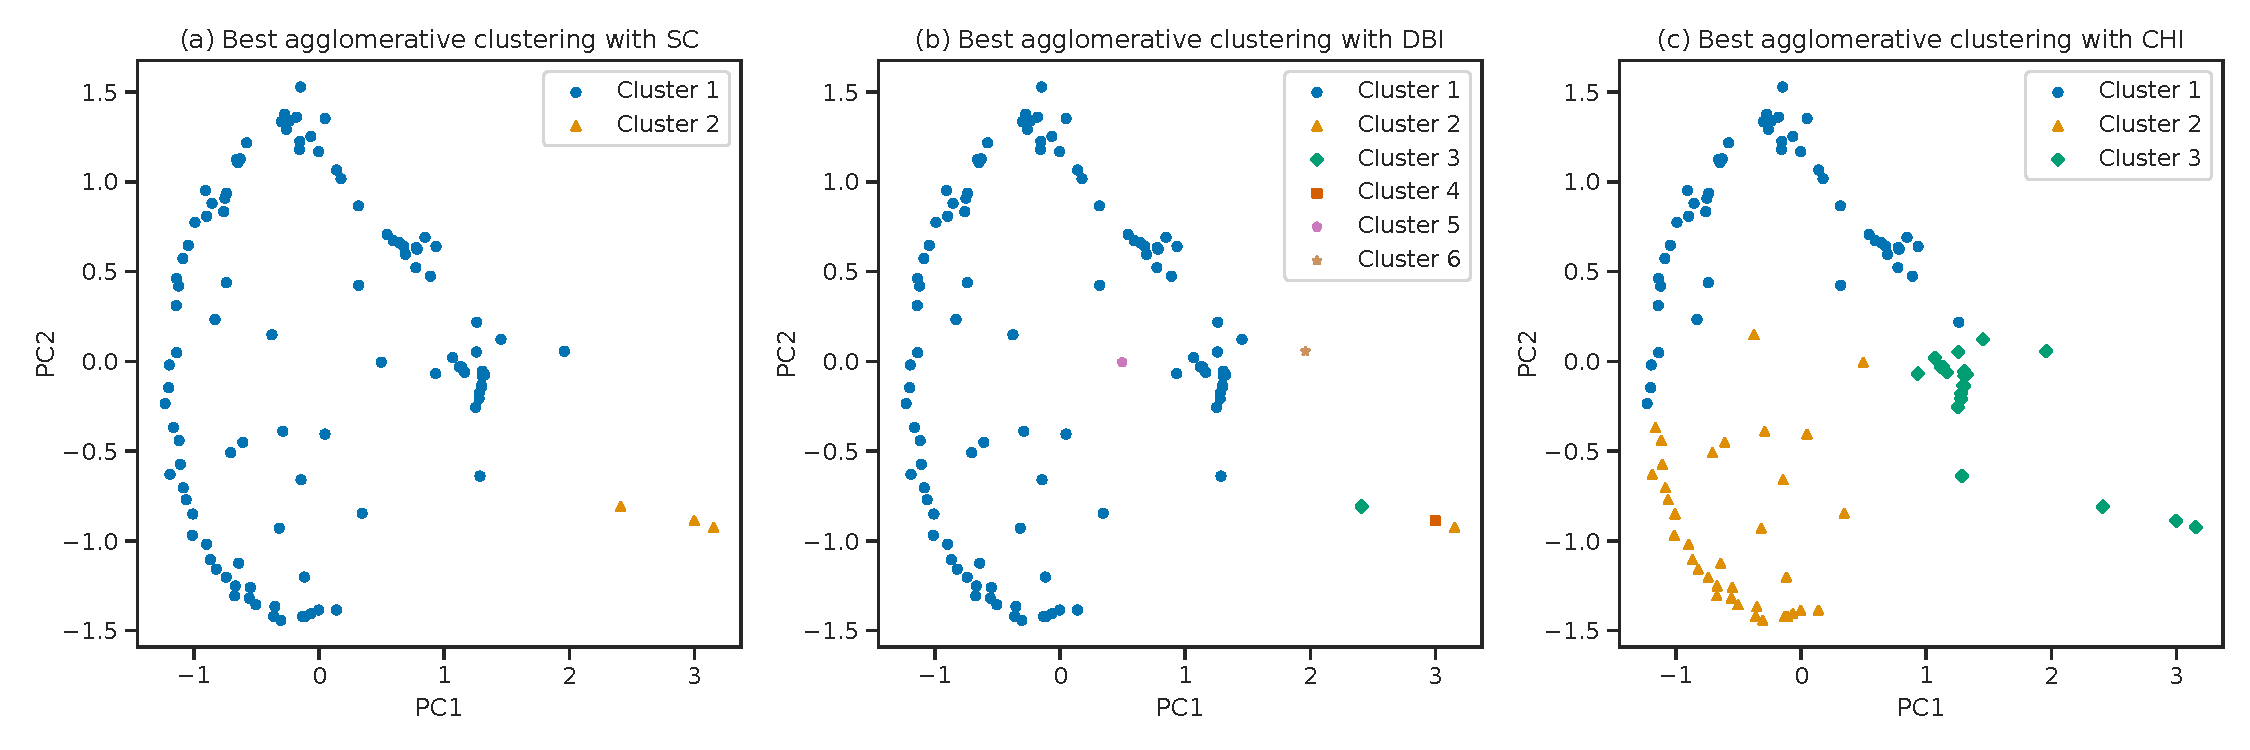
\includegraphics[width=\textwidth]{thesis/figures/cluster-analysis-agglomerative-numbers-word-group-internal-cluster-validation-best-2d-pca.pdf}
    \caption{Comparison of the best clustering results using agglomerative clustering on the number word embeddings of the SGNS-enwiki model. Here we see that it is not clear which clustering is the best.}
    \label{fig:cluster-analysis-agglomerative-numbers-word-group-internal-cluster-validation-best-2d-pca}
\end{figure}

We further investigated the structure of the 2-dimensional PCA embedding of the number words and noticed an interesting relationship. We illustrate this relationship in \cref{fig:ordered-number-word-embeddings-2d-pca}, which shows that by assigning an increasing label from the smallest and to the largest number, we get that the colour of the label gradually increases from the smallest label colour to the largest label colour. In other words, there seems to be an underlying sequential relationship in the number word embeddings. Furthermore, this suggests that the underlying structure of number word embeddings may contain information that we have not been able to find yet.
\begin{figure}[H]
    \centering
    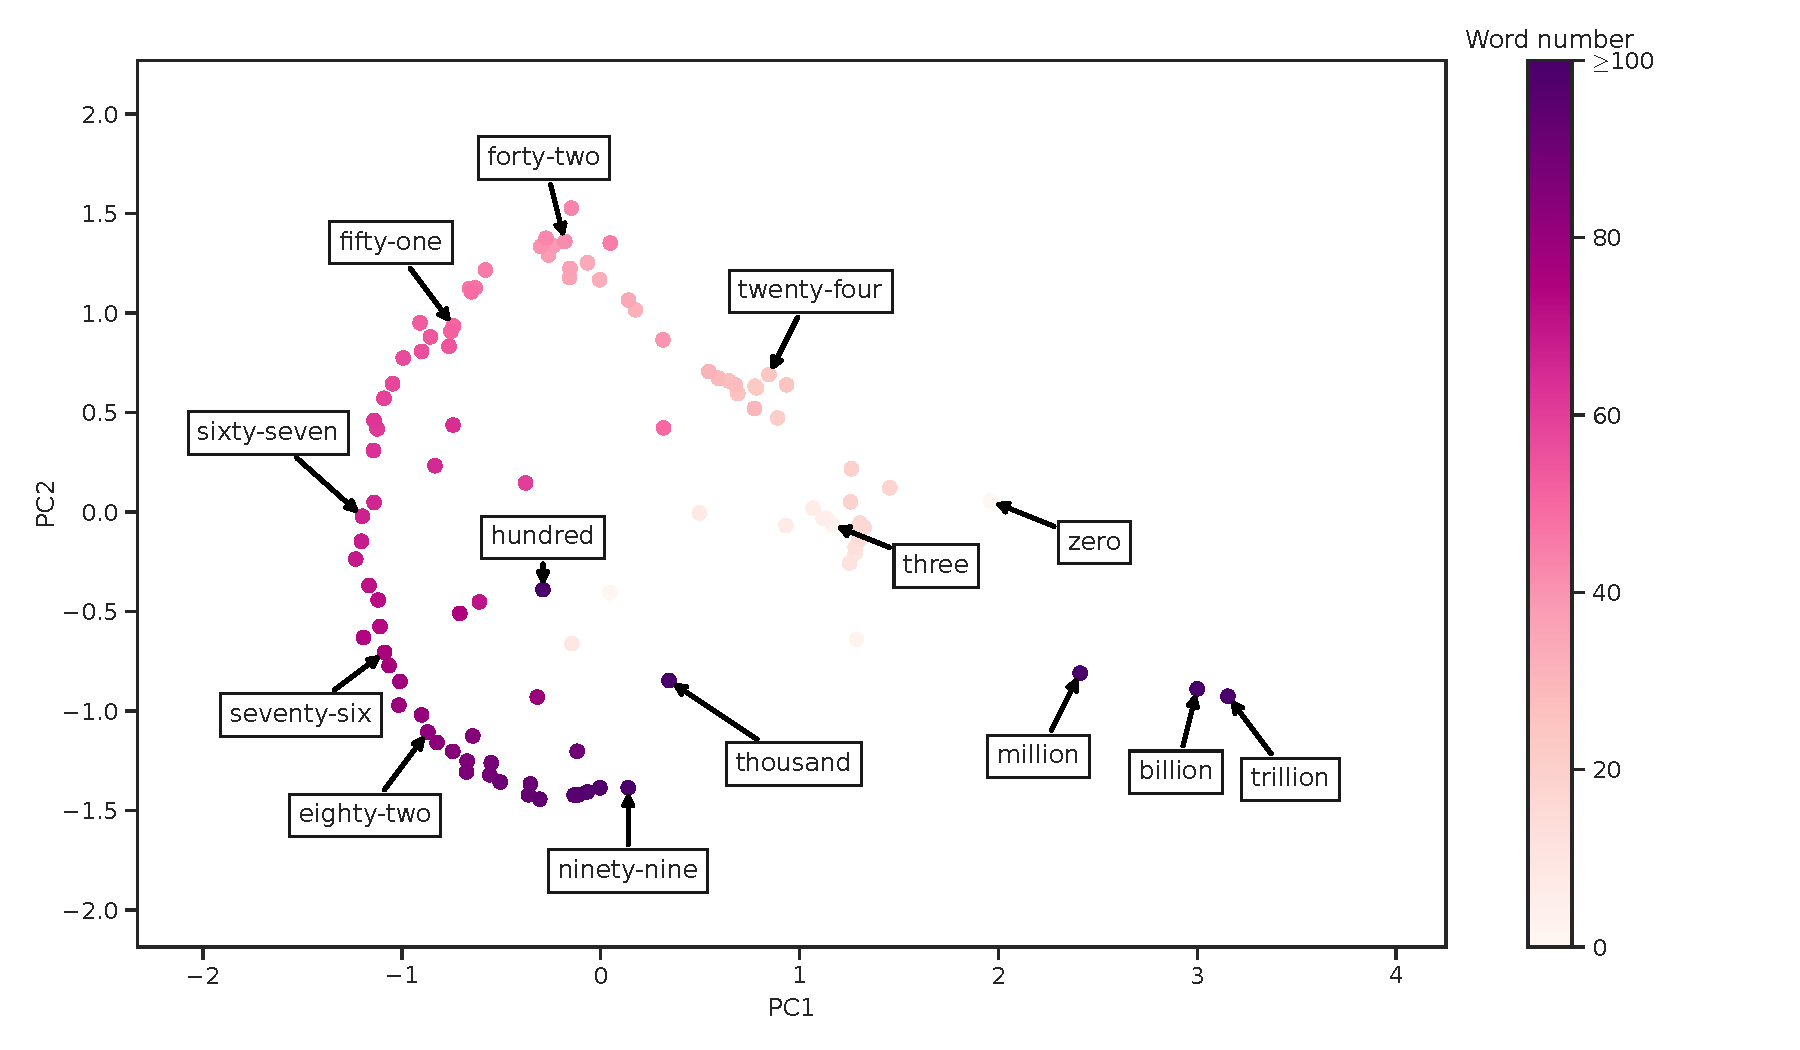
\includegraphics[width=\textwidth]{thesis/figures/ordered-number-word-embeddings-2d-pca.pdf}
    \caption{2-dimensional PCA embedding of the 105 number word embeddings, where each word embedding has an increasing label assigned to it. Here we see that as we increase the number, we see a possible underlying sequential relationship.}
    \label{fig:ordered-number-word-embeddings-2d-pca}
\end{figure}